\documentclass[conference]{IEEEtran}
\IEEEoverridecommandlockouts
% The preceding line is only needed to identify funding in the first footnote. If that is unneeded, please comment it out.

% test
\usepackage{amsmath,amssymb,amsfonts}
\usepackage{algorithmic}
\usepackage{graphicx}
\usepackage{textcomp}
\usepackage{xcolor}
\usepackage{lscape}
\usepackage{float}
\usepackage{multirow}
\usepackage{booktabs}
\usepackage{url}
\usepackage[numbers, sort]{natbib}
\def\BibTeX{{\rm B\kern-.05em{\sc i\kern-.025em b}\kern-.08em
		T\kern-.1667em\lower.7ex\hbox{E}\kern-.125emX}}

\newcommand{\boxedtext}[1]{\fbox{\scriptsize\bfseries\textsf{#1}}}
\newcommand{\nota}[2]{
	\boxedtext{#1}
	{\small$\blacktriangleright$\emph{\textsl{#2}}$\blacktriangleleft$}
}

\newcommand{\FIXME}[1]{{\color{red}\textsf{FIXME: #1}}}
\newcommand{\todo}[1]{{\color{red}\nota{TODO}{#1}}}
\newcommand{\fix}[1]{\textcolor{blue}{#1}}

\begin{document}
	
	\title{Achilles: Prioritizing Vulnerable Dependency Updates through Dependency Graphs}
	
	\author{\IEEEauthorblockN{Vipawan Jarukitpipat\textsuperscript{\textasteriskcentered}, Klinton Chhun\textsuperscript{\textasteriskcentered},
	Wachirayana Wanprasert\textsuperscript{\textasteriskcentered},
			Chaiyong Ragkhitwetsagul\textsuperscript{\textasteriskcentered}, \\
			Raula Gaikovina Kula\textsuperscript{\textdagger},
			Bodin Chinthanet\textsuperscript{\textdagger},
			Takashi Ishio\textsuperscript{\textdagger}, \\
			Morakot Choetkiertikul\textsuperscript{\textasteriskcentered}, 
			Thanwadee Sunetnanta\textsuperscript{\textasteriskcentered},
			Kenichi Matsumoto\textsuperscript{\textdagger}
		}
		\IEEEauthorblockA{\textsuperscript{\textasteriskcentered}\textit{Faculty of Information and Communication Technology (ICT), Mahidol University, Thailand} \\
			\textsuperscript{\textdagger}\textit{Nara Institute of Science and Technology (NAIST), Japan}\\
			\textit{Email: \{vipawan.jau, wachirayana.wan, klinton.chh}@student.mahidol.edu\}\\ 
			\textit{\{raula-k, bodin.chinthanet.ay1, ishio, matumoto\}@is.naist.jp},
			\textit{\{chaiyong.rag, morakot.cho, thanwadee.sun\}@mahidol.edu}
		}
	}
	\maketitle
	\thispagestyle{plain}
	\pagestyle{plain}
	
	\begin{abstract}
		The use of third-party dependencies in software applications is commonplace for contemporary software development, especially with the rise of available software library ecosystems like the Node.js packages (npm). 
		A key threat to the usage of third-party dependencies has been the threat of security vulnerabilities, which risks unwanted access to a user application. 
		Furthermore, as part of an ecosystem of dependencies, users of a library is prone to both the direct and indirect (transitives) dependencies that they have adopted into their application. 
		There has been recent work that involve tool support for vulnerable dependency updates, but the extent to which these tools aid the prioritization of dependency updates is unknown. 
		In this paper, we adopt a visual approach to understand how to support a developers decision to prioritize a vulnerable dependency update.
		As a prototype, we present \texttt{Achilles}, which is a tool that shows a visualization (i.e., using dependency graphs) of both direct and indirect dependencies that are affected by software vulnerability attacks.
		To evaluate the effectiveness of \texttt{Achilles}, we performed a user study against the state of the art tools (Dependabot and npm audit). 
		By having 20 participants to perform two tasks of prioritizing dependency vulnerabilities to fix, we found that 7 participants who used Achilles gave different prioritization from when using Dependabot report in both two tasks. This is higher than 4 and 6 participants who used npm audit.
		We show that there is a difference in using a visualization, as it provides more intuitive information on the complexity, and highlights the directs and indirect vulnerable dependencies when compared to the textual results of both Dependabot and npm audit.
		Our work provides insights into the what factors influence developers priorities when updating, and shows evidence that visual tool support is needed when deciding to update.
	\end{abstract}
	
	\begin{IEEEkeywords}
		software libraries, fixing known vulnerabilities, dependency graph, software visualization
	\end{IEEEkeywords}
	
	\section{Introduction}
	The use of third-party dependencies in software applications is now prevalent for contemporary software development. 
	Much of this is due to the rise of available software library ecosystems like the Node.js packages (npm), which now hosts over 1.6 million library packages and is relied upon by more than 11 million developers worldwide\footnote{\url{https://www.npmjs.com/}}.
	Furthermore, the importance of npm packages is evident in industry, by its purchased by Microsoft's GitHub in 2020\footnote{https://github.blog/2020-03-16-npm-is-joining-github/}.
	
	A key threat to the usage of third-party dependencies has been the threat of security vulnerabilities, which risks unwanted access to a user application. 
	Furthermore, as part of an ecosystem of dependencies, users of a library is prone to both the direct and indirect (transitives) dependencies that they have adopted into their application. 
	The typical response to security vulnerability is a security advisory, which lets developers know of the security threats. 
	For instance, the GitHub Advisory Database \footnote{\url{https://github.com/advisories}} contains a curated list of security vulnerabilities that have been mapped to packages tracked by the GitHub and stored in the Common Vulnerabilities and Exposures (CVE) format.
	The GitHub Advisory Database is sourced from the National Vulnerability Database (NVD)\footnote{\url{https://nvd.nist.gov/}} and the npm security advisories\footnote{\url{https://www.npmjs.com/advisories}}.
	
	Together with security advisories, there has been recent work that involve tool support for vulnerable dependency updates.
	Two tools that have been prevalent and the state of the art is both Dependabot \cite{Web:github_dependabot} and npm audit \cite{Web:npm_audit}. 
	Both tools help developers, by identifying vulnerabilities in existing dependencies and automatically creates a Pull Request to update the dependencies. \todo{Only Dependabot creates a PR, not npm audit}
	Recent work from \citet{Alfadel:MSR2021} found that developers are highly receptive to pull requests from Dependabot.
	However, even with these tools, developers struggle to update their dependencies. 
	Prior studies showed that developers are slow in updating their dependencies \citep{Robbes:2012, Hora:2015, Sawant2016, Bavota:2015, Ihara:2017}, due to various factors such as compatibility issues, being unaware and the migration effort outweighing the benefits.
	Kula et. al \cite{Kula2018} find that most developers were unaware of dependency updates, but also cited other issues such as the migration effort as a barrier to adopting a dependency update.
	Although existing tools exist to provide a fix, the extent to which developers prioritize which security updates should be fixed is still unknown.
	
	In this paper, we adopt a visual approach to understand how developers can use more dependency information to prioritize their decisions on which vulnerable dependency to update. 
	We posit that given more information, \textit{are  developers more motivated to rationalize and prioritize their decisions to update?} 
	As a prototype, we present \texttt{Achilles}, which is a tool that shows a visualization (i.e., using dependency graphs) of both direct and indirect dependencies that are affected by software vulnerability attacks.
	To evaluate the effectiveness of \texttt{Achilles}, we performed a user study against the state-of-the-art tools (Dependabot and npm audit). 
	We recruited 20 participants to perform two tasks of prioritizing dependency vulnerabilities to fix and found that 7 participants who used Achilles gave different prioritization from when using Dependabot report in both two tasks. This is higher than 4 and 6 participants who used npm audit and gave different prioritization from when using Dependabot.
	
	We show that there is a difference in using a visualization, as it provides more intuitive information on the complexity, and highlights the direct and indirect vulnerable dependencies when compared to the textual results of both Dependabot and npm audit.
	Our work shows that  visual tool support is needed for prioritizing dependency updates.
	
	\section{Background and Basic Concepts}
	In this section, we show the list of prior works and key concepts related to dependencies, issues on dependency updating, and security vulnerabilities.
	
	\subsection{Library Dependencies}
	In contemporary software development, reusing code is a common practice. These reused code come in the form of software dependencies that developers can easily incorporate into their software project with only a single statement. This activity reduces the developers' effort in writing code from scratch and also avoid repeating steps in software development for such code including designing, writing, testing, debugging, and maintaining a specific unit of code~\cite{Cox2019}.
	
	\subsubsection{Direct vs.~Indirect Dependencies}
	A \textit{direct dependency} means a software dependency that is directly called from the developer's code. This type of dependencies are the dependencies that are listed in \texttt{include} or \texttt{import} statements or in a dependency file such as \texttt{package.json}. The direct dependencies usually contains functionalities that the developer wants to include in their software project and the calls to such functionalities can be found in the project code. 
	
	On the other hand, an \textit{indirect dependency} or \textit{transitive dependency} is a software dependency that is called from a direct dependency or an indirect dependency. Similar to the direct dependency, the indirect dependencies contain functionalities that the other dependencies require or depend on. The indirect dependencies can be created in different levels depending on how many dependency calls occur. A thread of all the dependencies that depend on each other from the project to the dependency in the last level can be called a \textit{dependency chain}. 
	One direct dependency can also create several indirect dependencies of the same level by calling several other dependencies in their code. Previous study~\cite{Zimmermann2019} shows that there are approximately 80 indirect dependencies per one direct dependencies installed and the trend is increasing over time. This large number of indirect dependencies and their invisibility from the developer's point of view can result in difficulty in locating flaws or vulnerabilities introduced to the software project by the indirect dependencies~\cite{Cox2019}.
	
	\subsection{Developer Struggles with Updating}
    % The new release of dependencies introduces new features and fixes for \todo{incomplete sentence?}. 
    Updating dependency is an important task in the software development as it introduces new features and bug fixes.
    Despite being important, prior studies showed that developers are slow in updating their dependencies.
    \citep{Robbes:2012, Hora:2015, Sawant2016, Bavota:2015, Ihara:2017}. 
    %\todo{Bodin please expand}
    
    \citet{Robbes:2012} and \citet{Sawant2016} studied on how developers react to the deprecated API.
    They found that only a minority of software project updates their API and tends to use the older version instead.
    \citet{Bavota:2015} studies the dependency updates in the Apache community.
    They found that developers are unwilling to update the dependencies, if some APIs are removed.
	\citet{Decan:2017} investigated the evolution and issues of dependency from different ecosystems.
	They revealed that these ecosystems have the issue with dependency update.
	This issue is not only affect to the direct user of dependencies, but it is also transitively to indirect user of these dependencies.
    \citet{Ihara:2017} empirically showed software projects do not always use the latest version of dependencies.
	\citet{Bogart:2015} conducted a survey and found that developers prefer to keep outdated dependencies as the new version might breaks their code.
	\citet{Kula:2017} found that updating dependencies task is influenced by the amount of effort needed to change the API in the application.
	The important updates such as vulnerability fix and new major version that introduce new features are also influence how long developers need to adopt these updates.
	\citet{Decan:ICSME:2018} conducted an empirical study of technical lag in the npm ecosystem and found that the lags occur as the semantic versions of dependencies are not cover the latest release.
	They also found that using proper semantic versioning could reduces the technical lag.
	\citet{Chinthanet2021} focused on the lags of update in the case of vulnerability fix releases in npm ecosystem.
	They confirmed that despite the size of vulnerability fixes is small in terms of commit, developers still have a slow reaction to those fixes which cause lags of updates through out the dependency network.
	They also find that the severity of vulnerabilities is one of the factors that influences lags.
	
	\subsection{Analyzing and Fixing Vulnerable Dependencies}
	    Nowadays, there are automated tools that can help developers analyzing dependency security vulnerabilities in their software project. Two tools that are widely used include GitHub Dependabot and npm audit. We explain each of them below.
		
	\subsubsection{GitHub Dependabot}
	In 2019, GitHub acquired Dependabot, the bot that automatically creates the pull requests to keep dependencies secure and up-to-date for GitHub repository.
	Dependabot currently supports repository written in 15 languages.
	The process of Dependabot consists of three steps: (i) the bot finds outdated or vulnerable dependencies, (ii) the bot opens a pull request for each dependency, and (iii) the developers check the changes and merge them to the repository.
	% The recent work from Alfadel et. al. investigated the degree to which developers adopt the bot in their repositories \cite{Alfadel:MSR2021}.
	% They found that developers are highly receptive to pull requests from Dependabot.
	However, the limitation of Dependabot is that it cannot detect vulnerability from indirect dependencies.\footnote{\url{https://github.com/Dependabot/Dependabot-core/issues/2640}}
	\subsubsection{npm-audit}
	In 2018, npm introduced the new command for assessing the vulnerability from npm package dependencies called npm-audit.
	The command submits the list of dependencies from package.json file to the npm registry for a vulnerability report.
	Node.js developers could receive the vulnerability report while installing the dependencies from npm by default.
	Developers are also able to call npm-audit manually when they need.
	
	\begin{figure*}[tb]
		\centering
		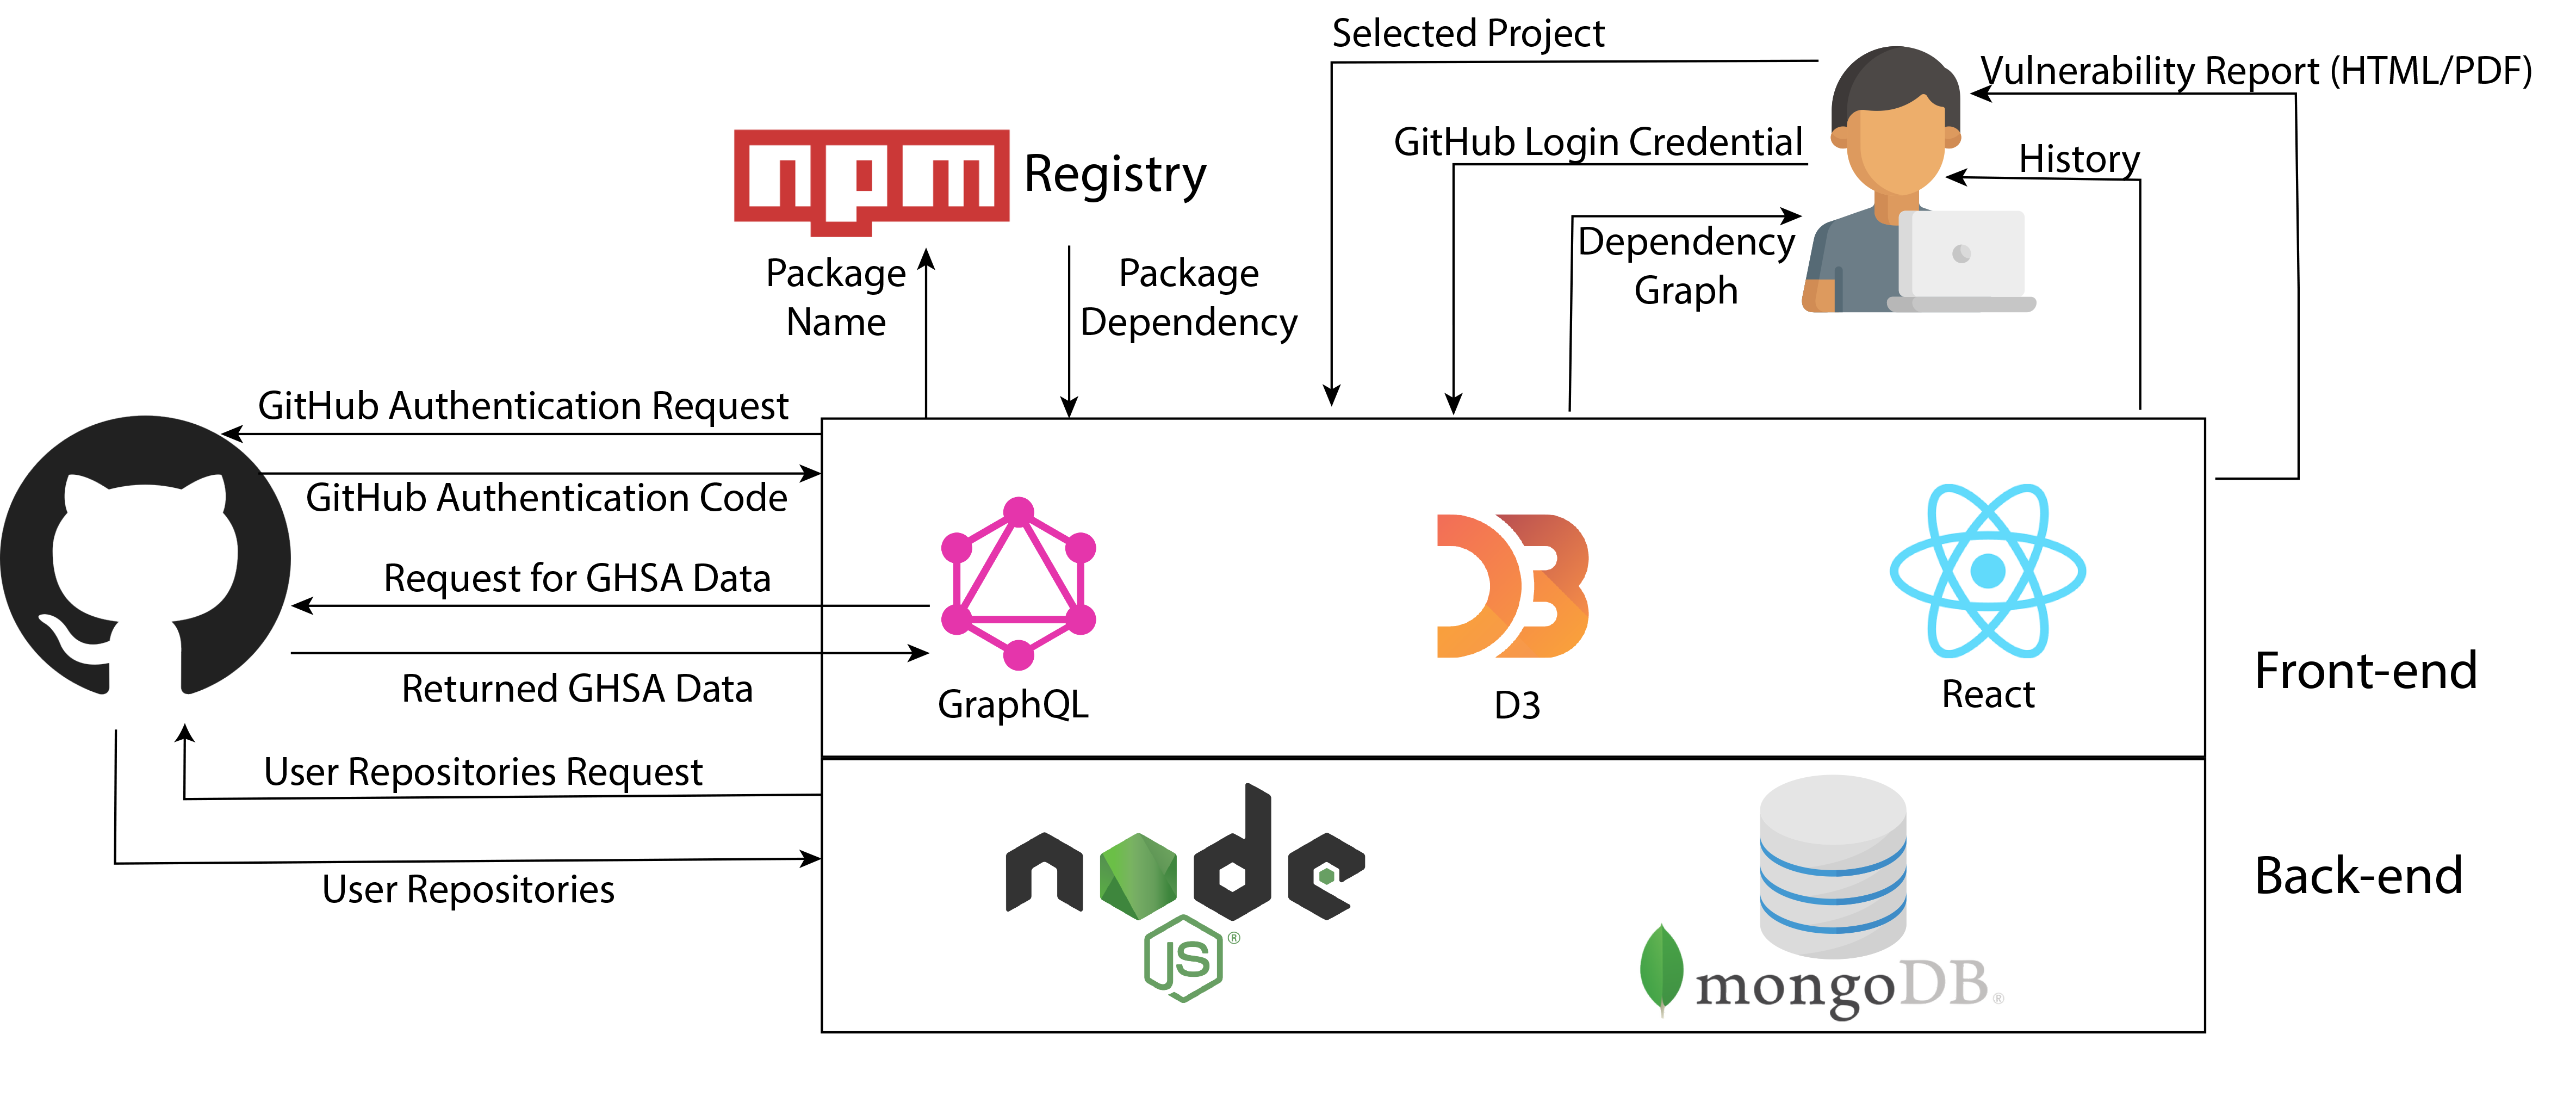
\includegraphics[width=1.2\columnwidth]{Figures/SystemArch.png}
		\caption{System Architecture of Achilles}
		\label{fig:system_architecture}
	\end{figure*}
	
	\section{Achilles}
	In this section, we present our prototype tool that is able to visualize, and provide more information, which has potential for a developer to prioritize their dependency updates. 
	
	\subsection{Technologies and Walk-through Design}

	As shown in Figure~\ref{fig:system_architecture}, we create a web-based prototype tool called ``\texttt{Achilles}''\footnote{The name \texttt{Achilles} has been chosen as a metaphor of Achilles' heel, which represents a weakness in a software project.} for demonstrating the concept of dependency graph visualization. \texttt{Achilles} connects to GitHub and retrieves the user's npm repositories. It then analyzes the repository's dependencies and produces the dependency graph visualization and a security analysis report.  the tool consists of the front-end and the back-end parts. The front-end part consist of GraphQL, D3, and React frameworks. The back-end parts consists of Node.js and MongoDB Atlas database.

    The \texttt{Achilles} tool analyzes security vulnerabilities in an npm project and creates a dependency graph visualization as follows.
    First, React library handles the user interface and interactions with the users. After a user login with his or her GitHub account, Node.js is used to query the user's list of repositories. After the user selects a package.json file which contains the list of npm dependencies, \texttt{Achilles} analyzes the relationships between the project and their packages using the data from the selected package.json file. This is when the tool gets the first level of dependencies. Then, \texttt{Achilles}  uses the list of first-level dependencies to send requests to the npm registry to retrieve other levels of dependencies using GraphQL. Currently, \texttt{Achilles} can retrieve dependency information up to 4 levels.
    After that, the chain of dependencies information is used to build a dependency graph using D3.js. The dependency graph visualizes the relationships between the project and its direct and indirect dependencies.
    
    Second, the analysis of dependency security vulnerability is performed by visiting each node in the graph and checking if its chain of dependency is vulnerable. The tool queries vulnerability information from GitHub Advisory Database\footnote{https://github.com/advisories} using GraphQL. 
    
    Lastly, we also make use of the interactions of web interface provided by JavaScript and the D3 library to display the dependency's vulnerability information as a tool tip. The tool tip information is only displayed when a user hovers the cursor over a node in the graph.
    Thus \texttt{Achilless} only shows relevant information that the user is interested in. 
    % If one of the nodes in the chain has found to be vulnerable, all the dependencies in that chain are marked as \textit{potentially vulnerable} by changing the node's color to red.
    % The edges connecting such nodes are also highlighted in red. Finally, the tool keeps the user's analysis history in MongoDB Atlas database.
        
    %In Achilles software system architecture (Figure \ref{fig:system_architecture}), we chose MongoDB Atlas database to store user and report information. We decided to choose this database because the data structure of the report that we need to store in database has various form of data such as vulnerable chaining node and vulnerability information that we get from GitHub Security Advisory which is returning JSON format. Moreover, MongoDB Atlas can store the data that is similar to the objects in the applications which benefits in reducing time in the need of translating the form of data that is stored in the database and the the form of data that is used in the code.

%Users can interact with the Achilles software to see the visualization of the dependency graph via the website, which we developed using React, a front-end framework for developing a website, and D3.js library, which is used to create the visualization. Public GitHub repositories can be retrieved without any authorization. However, users are required to sign in with GitHub in order to allow our system to access their private repositories.

%The Achilles software is developed using node.js to query data from MongoDB, get the users’ authentication from GitHub, retrieve users’ repositories information, and retrieve the package.json file.
	\begin{figure}
		\centering
		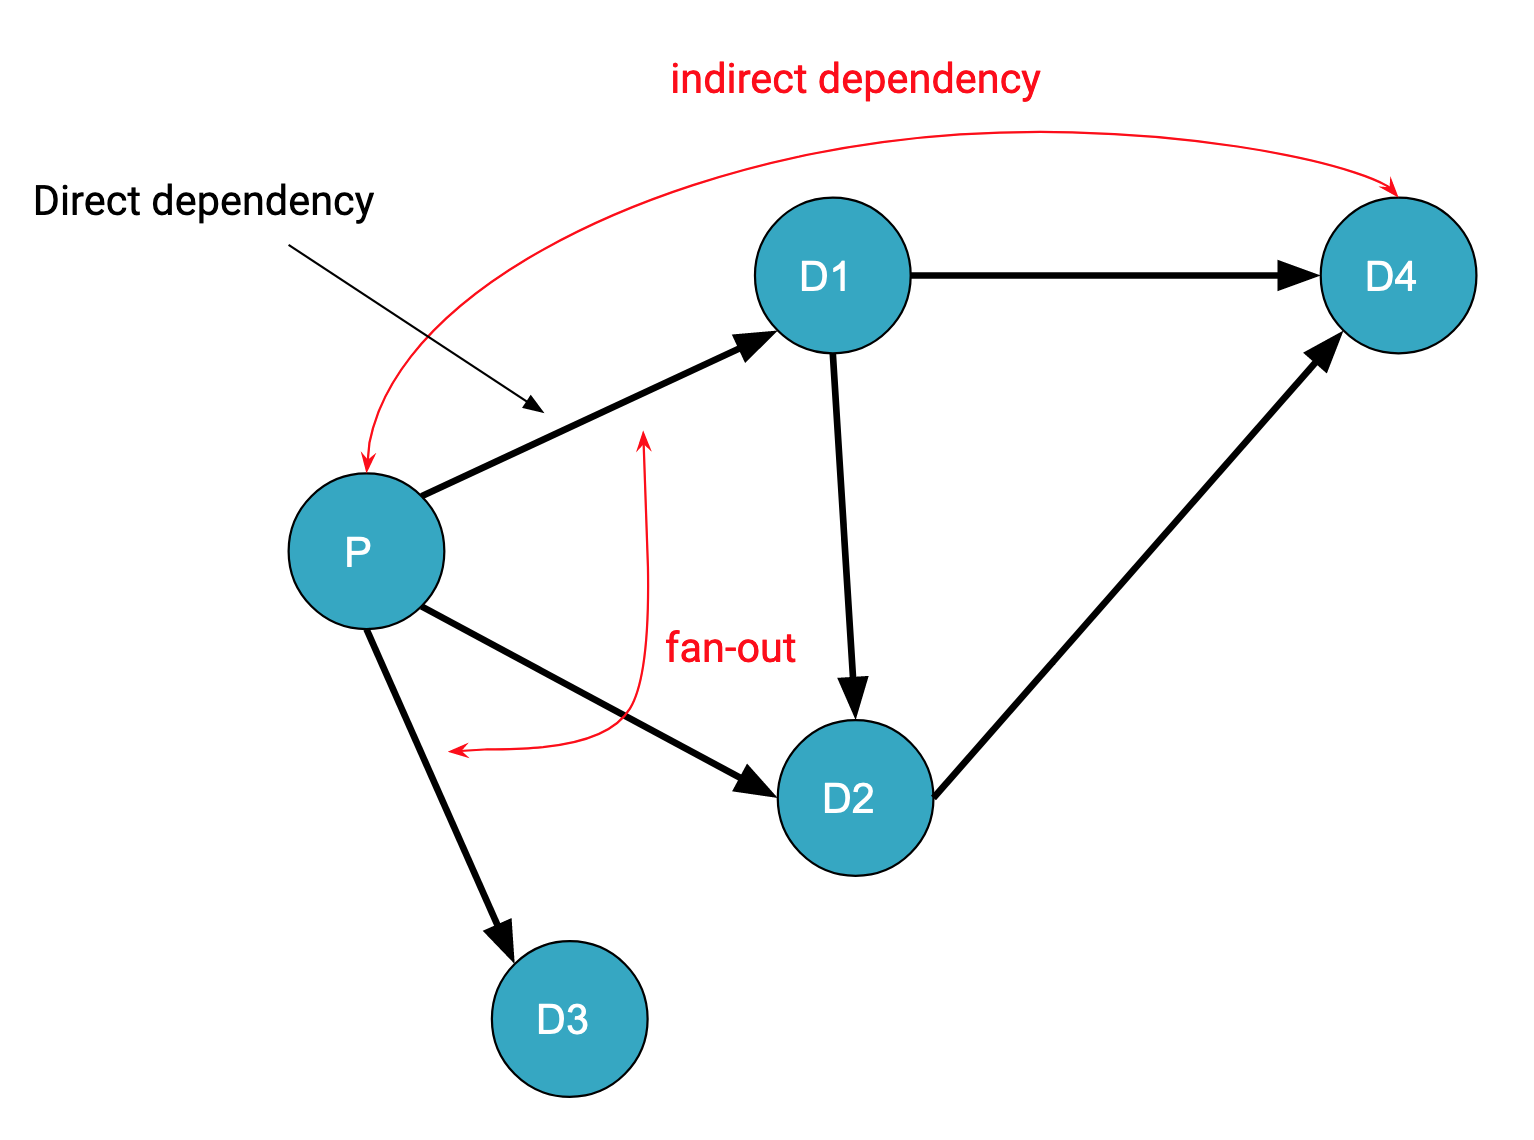
\includegraphics[width=0.9\linewidth]{Figures/Viz-concept-2}
		\caption{Using a dependency graph to depict direct and indirect dependencies.}
		\label{fig:viz-concept-2}
	\end{figure}
	
	\subsection{The Dependency Graph Visualization Design}
	Figure~\ref{fig:viz-concept-2} shows how we apply the graph visualization to npm dependencies.
	According to the concept presented by Herman et al.~\cite{Herman2000}, we found that the npm dependencies and their relationships match well with graph visualization. The graph visualization, the data can be represented by the nodes of a graph, with the edges representing their relations.
	
	\subsubsection{Direct and Indirect Dependencies.}
	\todo{use mathb for variables.} \todo{Like this $\mathbb{P}$? I tried and it looks different from the symbol used in the Figure}
	Since, dependencies in npm projects have a relationship between each other, we defined the node to represent a dependency (i.e., package in npm) and the edge to represent the usage of one dependency on the other.  Suppose that we have an npm project $\mathbb{P}$ which uses 3 dependencies, \textit{D1}, \textit{D2}, and \textit{D3}. Their relationship can be captured in a directed graph as shown in the figure. Node \textit{P} has an edge pointing to the node \textit{D1}, \textit{D2}, and \textit{D3} showing that it depends on these three dependencies. Moreover, the dependency \textit{D1} also depends on the existing dependency \textit{D2}, and a new dependency \textit{D4}. At the same time, \textit{D2} also depends on \textit{D4}. Thus, there are edges from the node \textit{D1} to \textit{D2} and to \textit{D4} and another edge from the node \textit{D2} to \textit{D4}. By establishing these relationships in the graph, we can easily identify the direct and indirect dependencies. The nodes that have the path length of 1 from the project node \textit{P} in the graph are direct dependencies. The rest are indirect dependencies. Furthermore, we can also see the fan-out of each node, i.e., how many dependencies such node have.  For example, in this figure, we can see that the project \textit{P} has a fan-out value of 3 by having 3 outgoing edges to \textit{D1}, \textit{D2}, and \textit{D3} respectively.
	


	\subsubsection{Colors}
	Figure~\ref{fig:viz-concept} shows how we represent the status each dependency using colors.
	The vulnerable nodes are shown in red to make them easily distinguishable from the others. The normal nodes are shown in different colors according to their levels in the dependency chain, i.e., how many hops they are from the project node. 
	\todo{I dont understand what is levels. This seems important} \todo{Would this additional explanation work?}
	We call the nodes with the path length of 1, 2, 3, and 4 from the project node as level 1, level 2, level 3, and level 4 respectively. The level-1 nodes or the direct dependencies are shown in light blue. The level-2 nodes are shown in dark blue. The level-3 nodes are shown in green and the level-4 nodes are shown in yellow. This use of different colors for each level helps to locate the dependencies that are in the same or different level.
	
	In addition, we also shown the edges that belong to a dependency chain which contains a vulnerable node in red. So, all the dependencies in the vulnerable dependency chain can be easily located. On the other hand, normal dependency chains have black-color edges.
	
	\begin{figure}[tb]
		\centering
		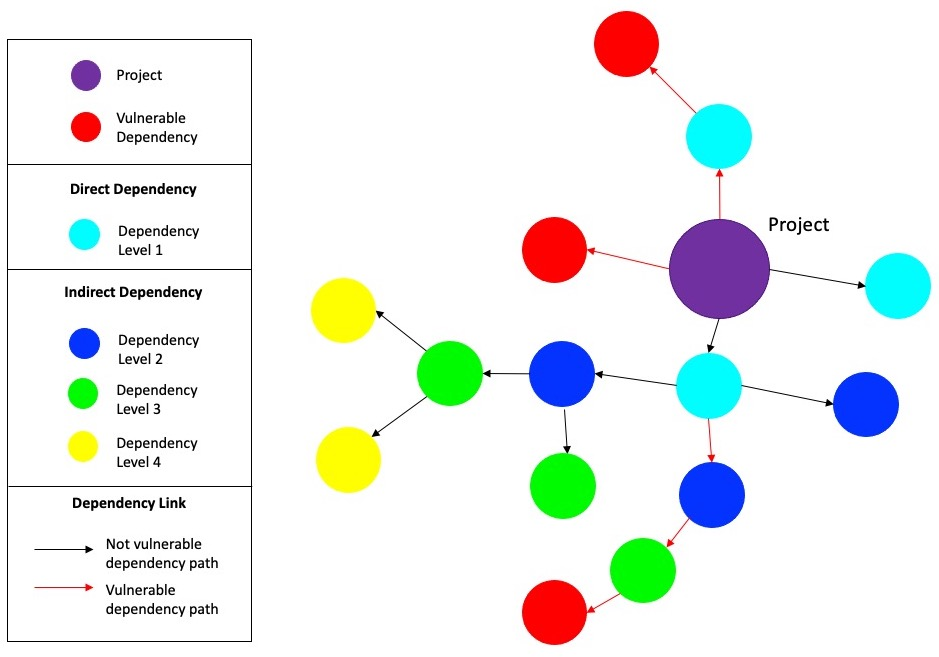
\includegraphics[width=\columnwidth]{Figures/Viz-concept-1.jpg}
		\caption{Meaning of node and edge colors in the dependency graph visualization}
		\label{fig:viz-concept}
	\end{figure}

\begin{figure}
		\centering
		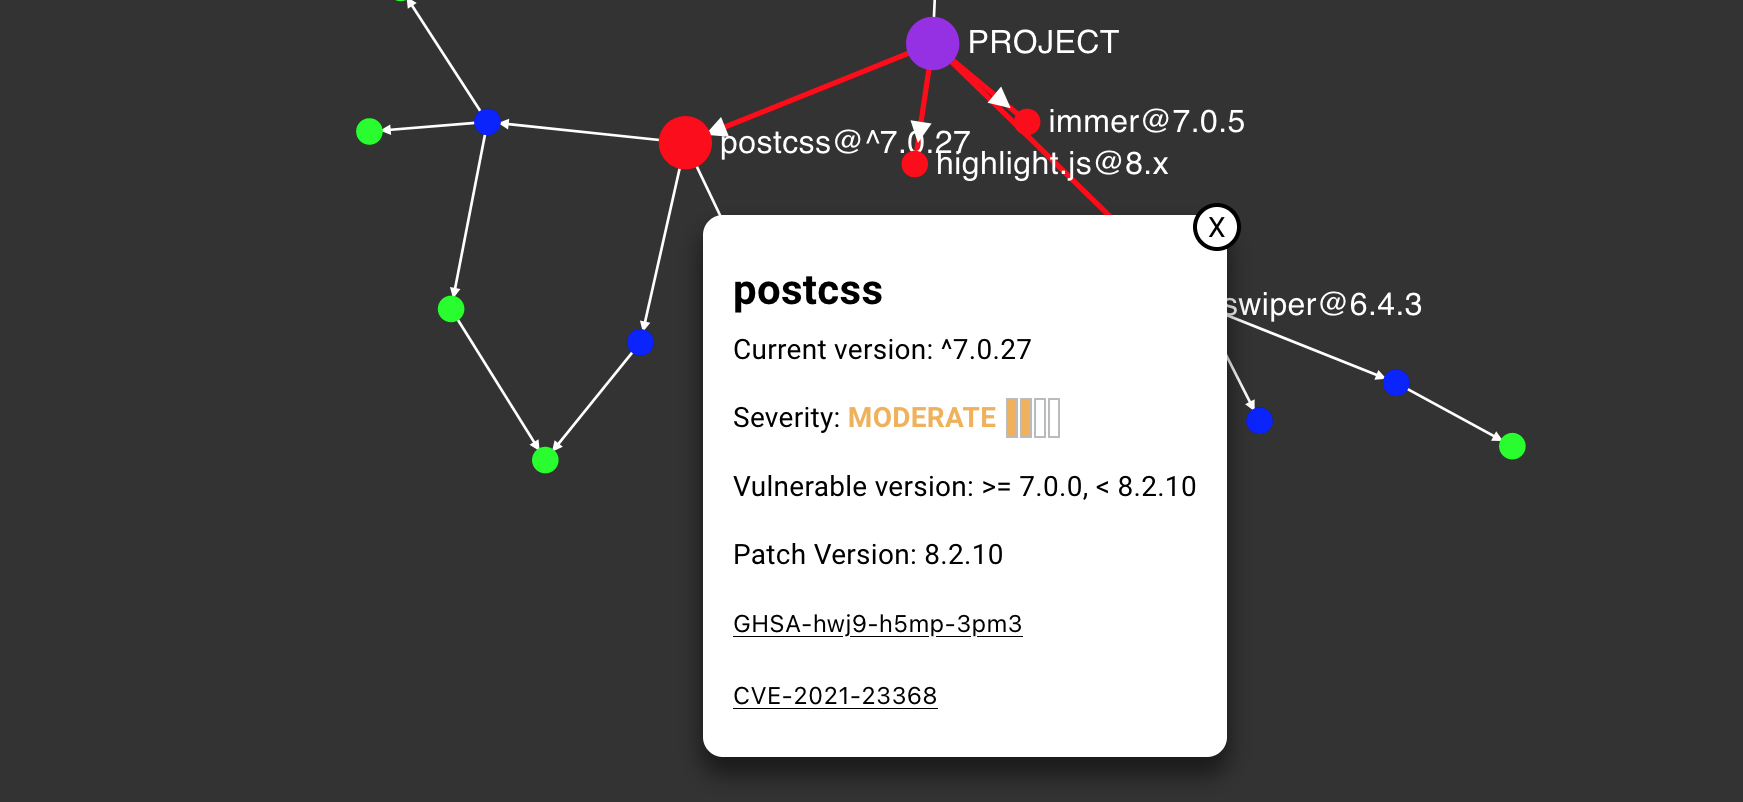
\includegraphics[width=\columnwidth]{Figures/tooltip_moderate}
		\caption{Vulnerable node: A tool tip that shows the dependency's vulnerability information}
		\label{fig:tooltip_moderate}
	\end{figure}

	\begin{figure}
		\centering
		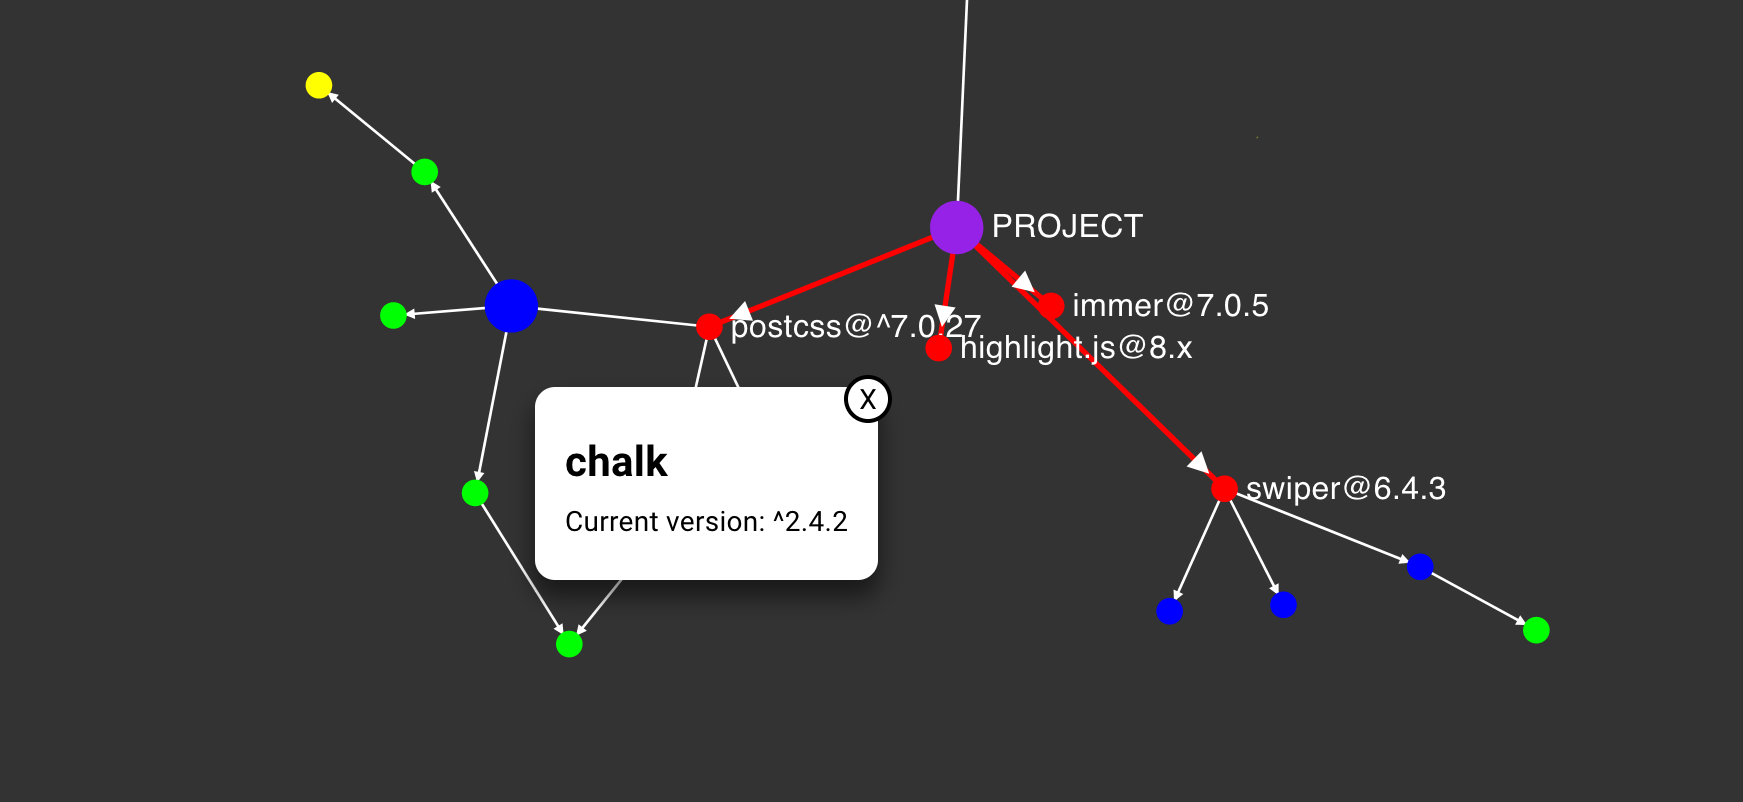
\includegraphics[width=\linewidth]{Figures/tooltip_normal}
		\caption{Normal node: A tool tip that shows the version of dependency}
		\label{fig:tooltip_normal}
	\end{figure}


	\begin{figure}[tb]
		\centering
		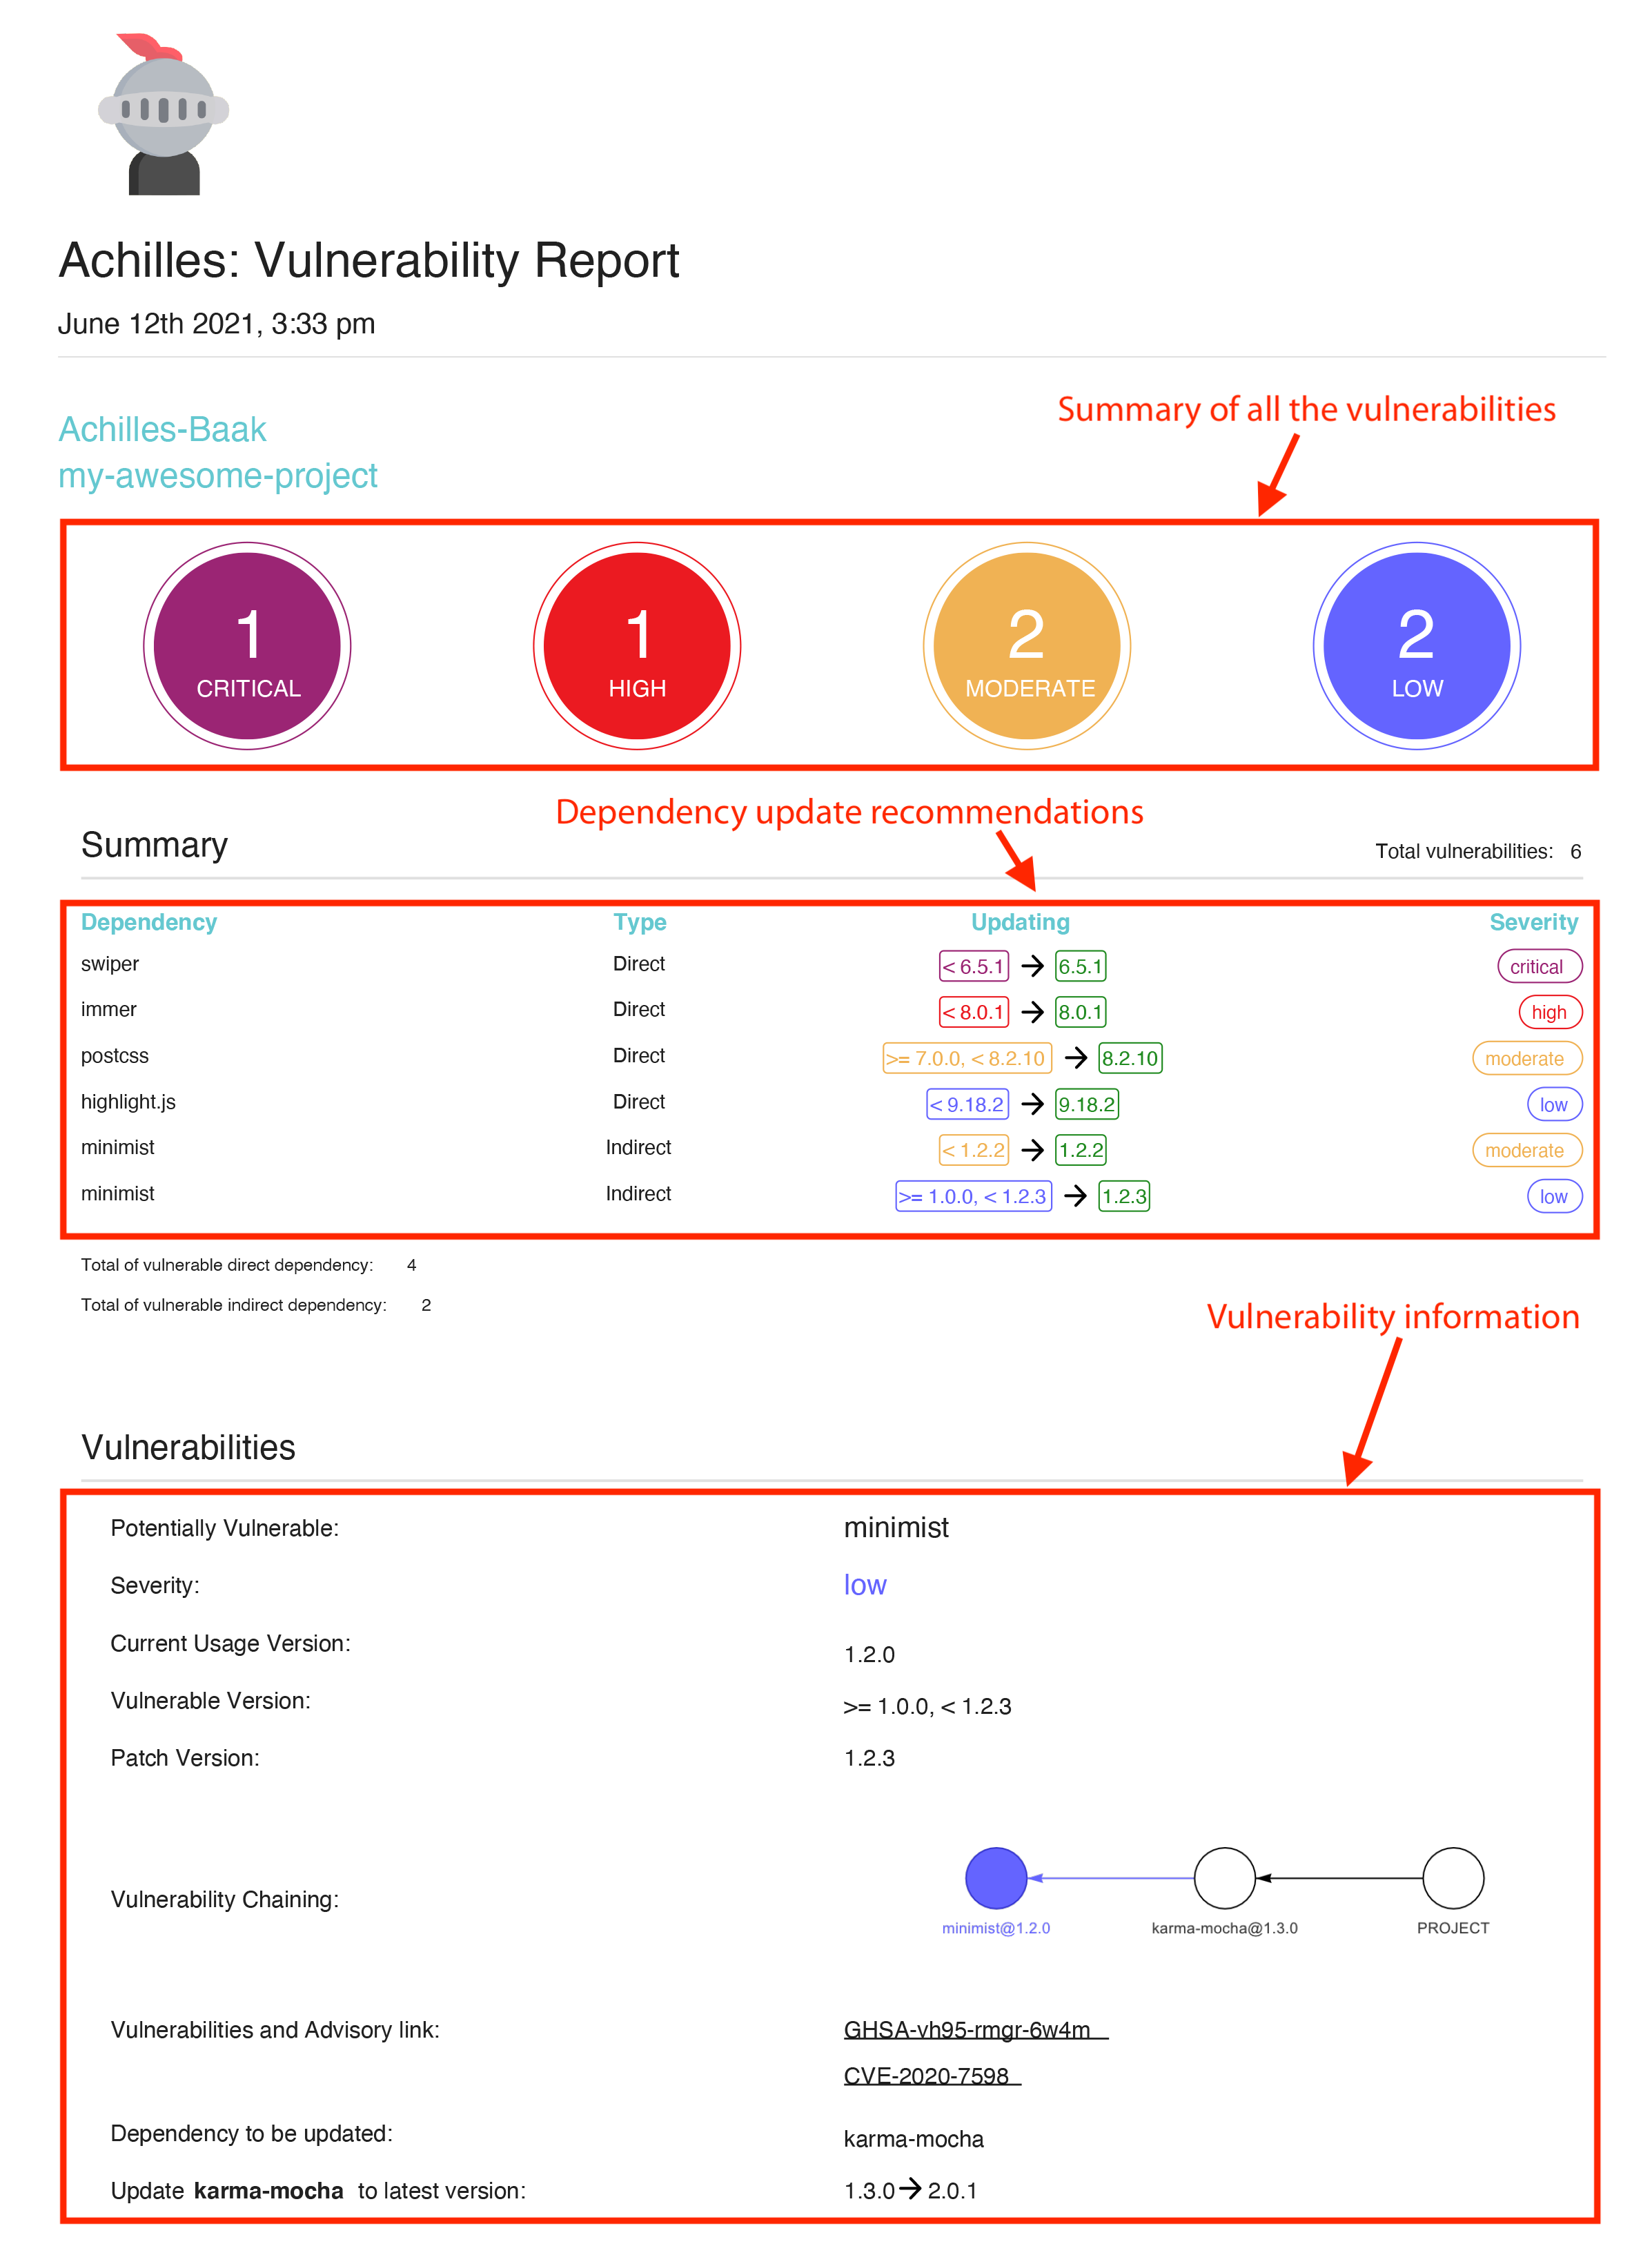
\includegraphics[width=\columnwidth]{Figures/my-awesome-project-achilles-report-1.png}
		\caption{\texttt{Achilles} vulnerability report}
		\label{fig:vul-report-1}
	\end{figure}
	
	\subsubsection{Tool Tip for Displaying Dependency's Vulnerability Information}
	Figure~\ref{fig:tooltip_moderate} and Figure~\ref{fig:tooltip_normal} show examples of the tool tip. If the hovered node is vulnerable, \texttt{Achilles} shows a tool tip with the information of the vulnerability, which include the dependency version in the project, its vulnerability severity (low, medium, high, critical), the range of the versions that are affected by the vulnerability, the patch version of this vulnerability, and the links to the vulnerability's CVE record in GitHub Advisory Database and in the National Vulnerability Database (NVD).
	\todo{CVE and GSAD is introduced too late, please explain in intro $\rightarrow$ Added. Please check.}
	The user can use this information for their further investigation of the vulnerability and support their decision on making updates. For normal nodes, the tool tip shows the version of the dependency (as shown in Figure~\ref{fig:tooltip_normal}).

	\subsubsection{The Vulnerability Report}
	As shown in Figure~\ref{fig:vul-report-1}, a vulnerability report can ge generated after the analysis of the dependency vulnerabilities is done. The report shows the summary of all the security vulnerabilities found in the analyzed npm project. As shown in Figure~\ref{fig:vul-report-1}, the report contains the summary of all the vulnerabilities found categorized by their severity levels on the top. 
	It also shows the recommendation of updating the vulnerabilities to the patch versions. Lastly, the remaining part of the report contains detailed information of each vulnerability similar to the information displayed in the tool tip. 
	A graph showing the dependency chain of the vulnerability is also included along with the link to the corresponding GitHub Advisory Database entry, the CVE record, and the CWE record (the type of software weakness introduced by the vulnerability) of such vulnerability. 
	The report can be saved for future references.

	
	\section{Evaluation Setup}
	We performed a user study to evaluate the effectiveness of the dependency graph visualization provided by \texttt{Achilles}.
	The objectives of the user study is to investigate how the dependency graph visualization supports developer’s decision on prioritizing vulnerabilities to fix and also to compare \texttt{Achilles} to the two state-of-the-art dependency vulnerability reporting tools: GitHub Dependabot and npm audit. 
	
	\subsection{Research Questions}
	We ask the following two research questions in this study.
	
	\begin{itemize}
		\item \textbf{RQ1: How does using a dependency graph visualization support developer’s decision on prioritizing vulnerability to fix?} In this RQ, we would like to study the effects of introducing the dependency graph visualization to the developers and how would the visualization supports the decision when the developers have to select or rank the security vulnerabilities to fix.
		\item \textbf{RQ2: How does using a dependency graph visualization perform compared to the state-of-the-art tools?} In this RQ, we want to compare the dependency graph visualization to the vulnerability report offered by the two state-of-the-art tools: Dependabot and npm audit.
	\end{itemize}
	
	\subsection{User Study Design}
	The user study follows the guidelines from \citet{Ko2013} and has been approved from the ethics committee. We highlight some of the key steps from the guidelines below.
	%, which consists of ten key steps including Recruitment, Selection, Consent, Procedure, Demographic measurements, Group assignment, Training, Tasks, Outcome measurements, and Debrief and compensate. We followed the guideline as shown below.
	
	\subsubsection{Recruitment and Selection}
	We set the inclusion criteria for selecting the participants of this experiment as follows:
	
	\begin{itemize}
		\item Participants must be computer science students or full-time employees at a software development company.
		\item Participants must have experience in programming for at least six months.
		\item Participants should understand and have fundamental knowledge in software vulnerabilities and related tools.
	\end{itemize}
	
	Then, we performed several methods to recruit the participants. For developers, we sent an email to invite them. For students, we recruited them by personal invitations. In total, we recruited 20 participants. We have listed their demographics, their experience on using npm, and whether they know indirect dependencies along with their assignments to the group in Table~\ref{table:participants}. Three participants were full-time developers. 6 participants were master's students and 11 participants were undergraduate students. Six participants were proficient in using npm and six participants knew about indirect dependencies before the study.
	
	\begin{table}[tb]
		\caption{Participants’ Demographic}
		\centering
		\resizebox{0.5\textwidth}{!}{%
			\begin{tabular}{lllp{1.1cm}p{1.1cm}}
				\toprule
				Group & Participants & Demographics  & npm Exp. & Know Ind.~Dep? \\ 
				\midrule
				Experimental & A1                                          & Master's student & Low & No \\ 
				& A2                                          & Master's student & High & Yes \\ 
				& A3                                          & Undergrad student & High & Yes \\ 
				& A4                                          & Developer & Low & No \\ 
				& A5                                          & Undergrad student & High & Yes \\
				& A6                                          & Undergrad student & High & No \\
				& A7                                          & Undergrad student & Low & No \\ 
				& A8                                          & Master's student & Low & No \\
				& A9                                          & Master's student & Low & No \\
				& A10                                         & Master's student & Low & No \\
				\midrule
				Controlled & N1                         & Master's student & High & Yes \\ 
				& N2                                          & Undergrad student & Low & No  \\ 
				& N3                                          & Developer & High & Yes \\
				& N4                                          & Undergrad student & Low & No \\
				& N5                                          & Undergrad student & Low & No \\
				& N6                                          & Undergrad student & Low & Yes \\
				& N7                                          & Undergrad student & Low & No \\
				& N8                                          & Undergrad student & Low & No \\
				& N9                                          & Undergrad student & Low & No \\
				& N10                                         & Developer & Low & No \\
				\bottomrule
			\end{tabular}
		}
		\label{table:participants}
	\end{table}
	
	\begin{table}[tb]
		\centering
		\caption{The participants' group assignment}
		\begin{tabular}{lrl}
			\toprule
			Group & Participants & Tools \\
			\midrule
			Controlled group & 10 & Dependabot $\rightarrow$ npm audit \\
			\midrule
			Experimental group & 10 & Dependabot $\rightarrow$ \texttt{Achilles} \\
			\bottomrule
		\end{tabular}
		\label{table:group_assignment}
	\end{table}
	
	\subsubsection{Group Assignment and Procedure}
	By following the between-subject experimental design~\citep{Charness2012}, we randomly assign the participants into two groups, (1) the controlled group and (2) the experimental group, as shown in Table~\ref{table:group_assignment}. The controlled group has ten participants. The participants in this group used npm audit to analyze security vulnerabilities. For the experimental group, the ten participants used dependency graph visualization provided by \texttt{Achilles} to analyze security vulnerabilities. 
	
	%The procedure of the user study between the controlled group and experimental group is as follows.
	We started by letting the participants read the consent form and ask for their confirmation to join the experiment. Then, we gathered their demographic background, provided the guidelines and videos of the tools demonstration, and asked them to perform two example tasks to train them to get used to the tools and security vulnerabilities in npm projects.
	
	%When the actual experiment began, both group of participants were asked to see the security vulnerability report from Dependabot and prioritize the updates of the vulnerabilities. Then, for the controlled group, they were asked to use npm audit. On the other hand, the experimental group were asked to use Achilles to find security vulnerability. After that the participants in the two groups were asked to prioritize the updates of the vulnerabilities again. Finally, we interviewed the participants on their criteria that they use for their prioritization.
	
%	\begin{figure}[tb]
%		\centering
%		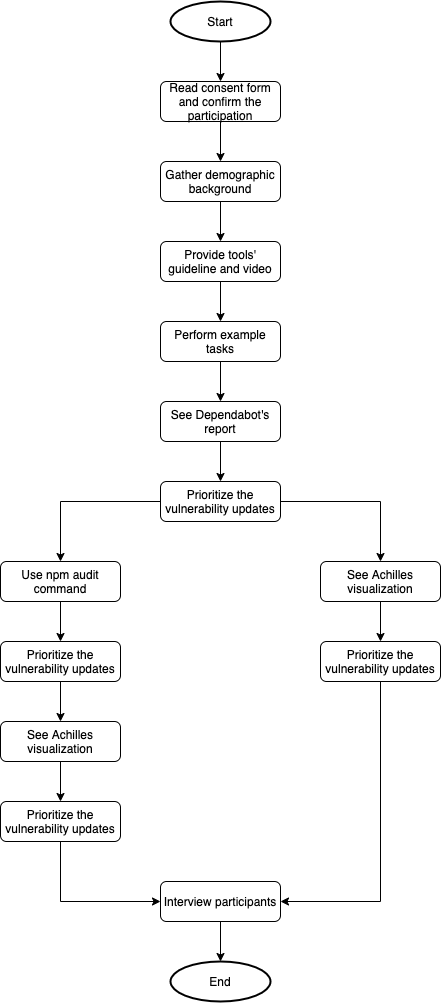
\includegraphics[scale=0.5]{Figures/fig1.png}
%		\caption{Procedures of User Study}
%		\label{fig:proceduresofuserstudy}
%	\end{figure}
	
	
	%\subsubsection{Demographic measurements} - We asked participants the following questions prior the experiment in order to gain more understanding of participants' background.
	%\begin{itemize}
	%         \item How long have you been using npm?
	%         \item What do you use npm for?
	%         \item How often do you check security vulnerabilities in the project?
	%         \item Do you know indirect dependencies?
	%\end{itemize}
	
	%\subsubsection{Training} - We provided the tools guidelines and videos for the tools demonstration. We also prepare example tasks to check their understanding of the tools before we begin the experiments.
	
	\begin{figure*}[ht!]
		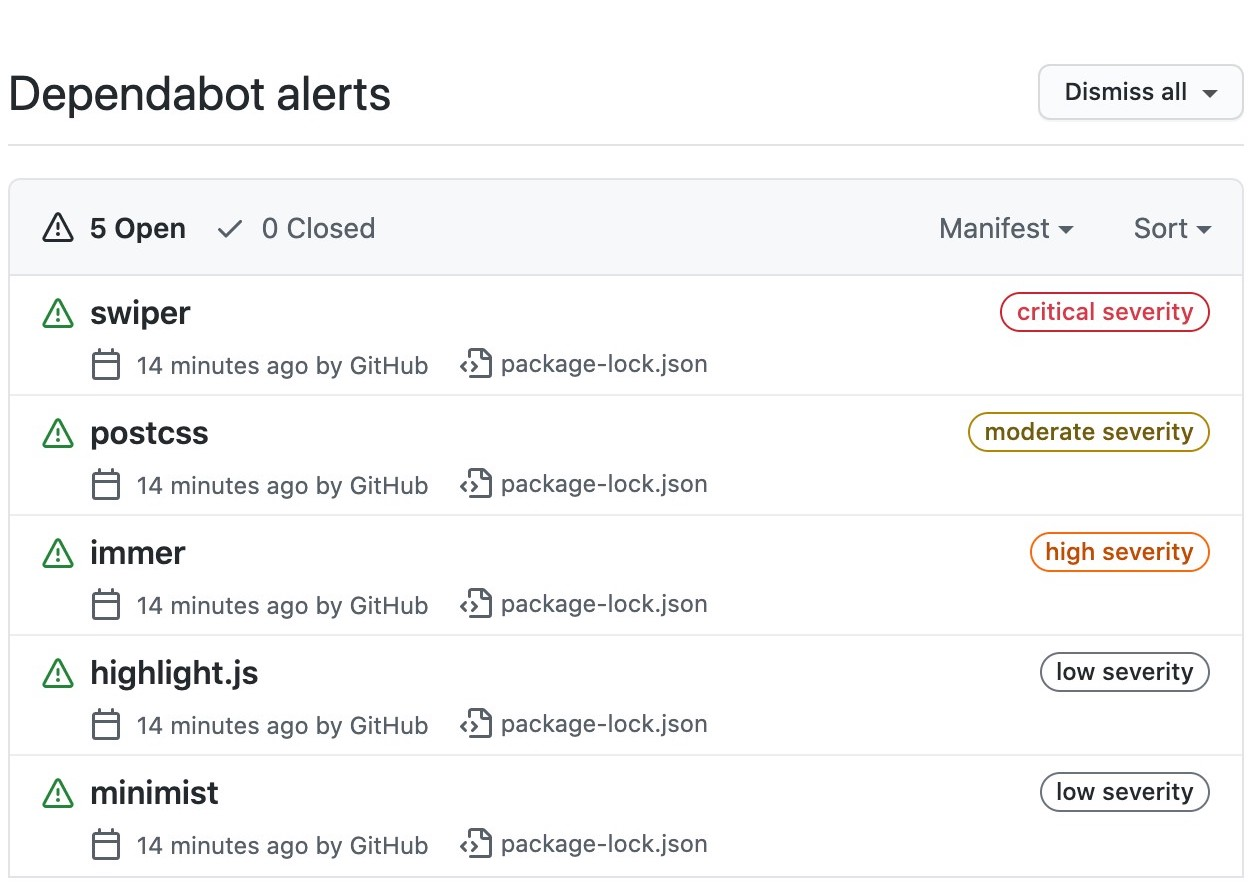
\includegraphics[width=.3\textwidth]{Figures/screenshot-dependabot.jpeg}\hfill
		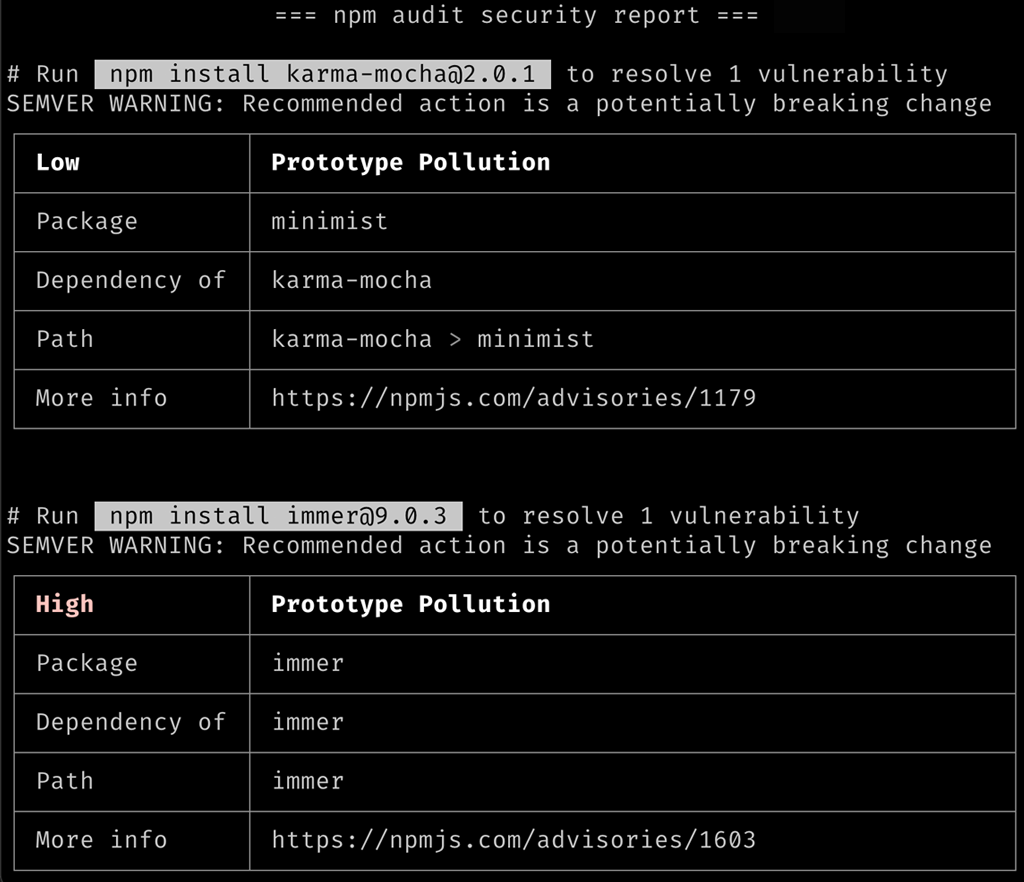
\includegraphics[width=.3\textwidth]{Figures/screenshot-npm-audit.png}\hfill
		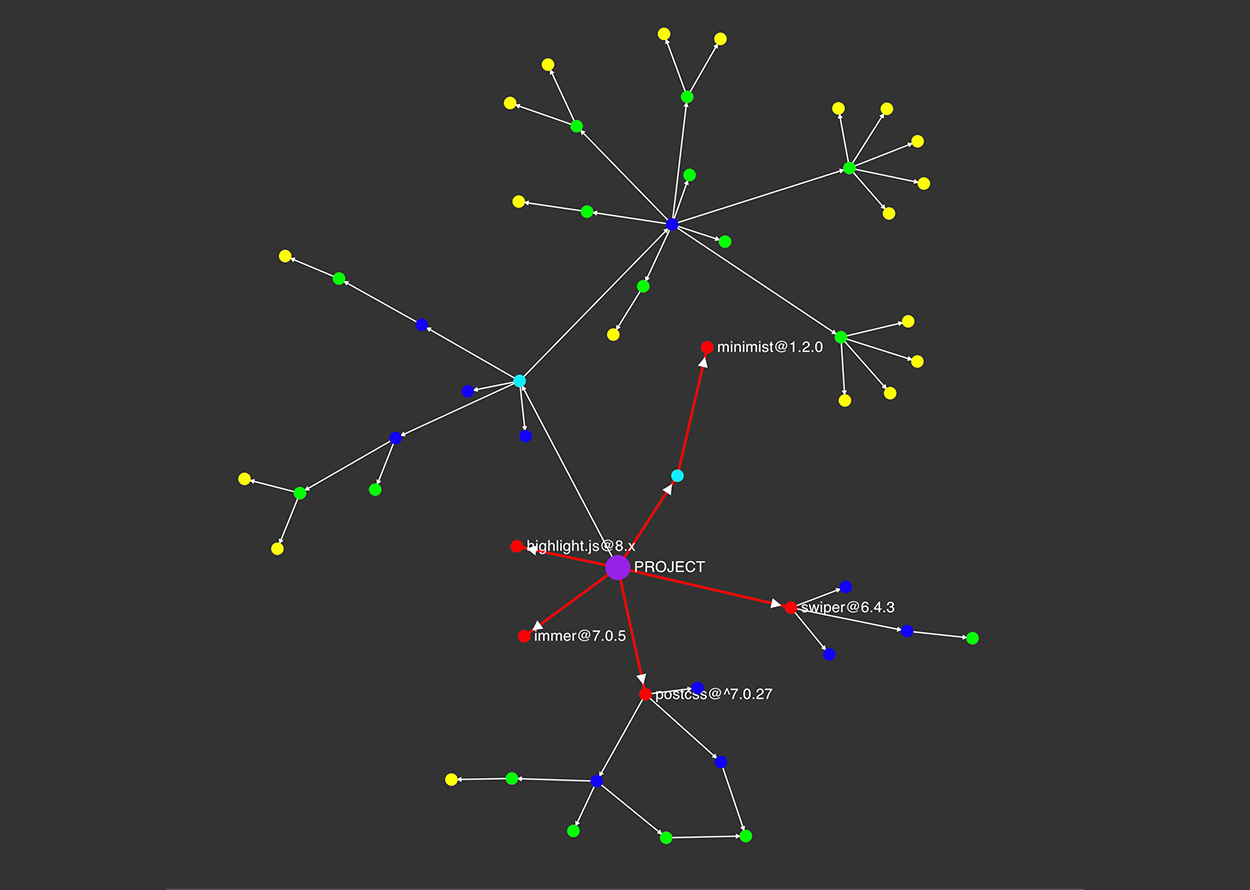
\includegraphics[width=.3\textwidth]{Figures/screenshot-achilles.png}
		\caption{The security report formats used in the user study produced by Dependabot (left), npm audit (middle), and \texttt{Achilles} (right)}
	\end{figure*}
	
	\subsubsection{Tasks} 
	The participants were asked to perform two tasks of prioritizing security vulnerabilities to fix in two npm projects. The participants needed to finish the first task before continuing to the second task.
	%The goal that they have to do is prioritizing the updates of the vulnerabilities after using each tool. 
	For each task, the participants had to do the following. Participants in both the controlled and the experimental groups were given an npm projrect and the vulnerability report of Dependabot. Then, they were asked to rank the vulnerable dependencies that they thought they would fix from the first to the last. After that, a different tool was introduced to each group. For the controlled group, npm audit was introduced. For the experimental group, \texttt{Achilles} was introduced. After using the given tool to explore the security vulnerabilities, the participants were asked to rank the vulnerable dependencies to fix again. 
	%Similarly for the experimental group, they were asked to see the vulnerability report of Dependabot in GitHub, rank the vulnerabilities to fix, use Achilles, and then rank again. 
	Additionally, we also asked the controlled group to see \texttt{Achilles} visualization after they had finished using npm audit. Then, they performed the dependency prioritization again.
	
	We call the two tasks that the participants had to perform \textit{Task 1 Vulnerabilities with Complex Dependencies} and \textit{Task 2 Vulnerabilities with Indirect Dependencies}. For Task 1, we aim to test whether the dependency graph visualization  would affect the participants’ decision on the dependency prioritization when the project contains ``complex'' dependencies. To achieve this, we created an npm project which contained 4 real-world vulnerable dependencies. We were interested in the dependencies which had different severity levels and also had different complexity levels. Thus, we selected two dependencies, \texttt{three} and \texttt{type-graphql}, that had high severity vulnerabilities and two dependencies, \texttt{xmldom} and \texttt{pug} that had low severity vulnerabilities. Two of the dependencies, \texttt{three} and \texttt{xmldom}, did not have any dependencies while the other two dependencies, \texttt{type-graphql} and \texttt{pug}, depended on a large number of dependencies, i.e., they introduced complexity into the dependency chain. 
	We made sure that the 4 selected dependencies could be detected by Dependabot, npm audit, and \texttt{Achilles}. Table~\ref{table:cha-teat1} shows the information of the dependencies in Task 1. The visualization of the dependencies in Tasks 1 is depicted in Figure \ref{fig:graphtest1}. 
	%\FIXME{which source of this level of vulnerabilities are from?} 
	From the visualization, we can see %the \texttt{three} and \texttt{xmldom} do not have any other dependencies. On the other hand, 
	that the 4 selected dependencies are direct dependencies of the project. Furthermore, \texttt{pug} directly depends on 8 other dependencies (highlighted with blue nodes) and \texttt{type-graphql} directly depend on 9 other dependencies. Their direct dependencies also depend on several other dependencies (green and yellow nodes).
	
	\begin{table}[tb]
		\centering
		\caption{Task 1: Vulnerabilities with Complex Dependencies}
		\begin{tabular}{llcccc}
			\toprule
			No & Dependency & Version & Severity & Type & Category \\
			\midrule
			1 & three & 0.12.40 & High & Simple & HS \\
			2 & pug & 2.0.4 & High & Complex &  HC \\
			3 & xmldom & \^{}0.4.0 & Low & Simple & LS \\
			4 & type-graphql & 0.17.5 & Low & Complex & LC \\
			\bottomrule
		\end{tabular}
		\label{table:cha-teat1}
	\end{table}
	
	\begin{figure}[tb]
		\centering
		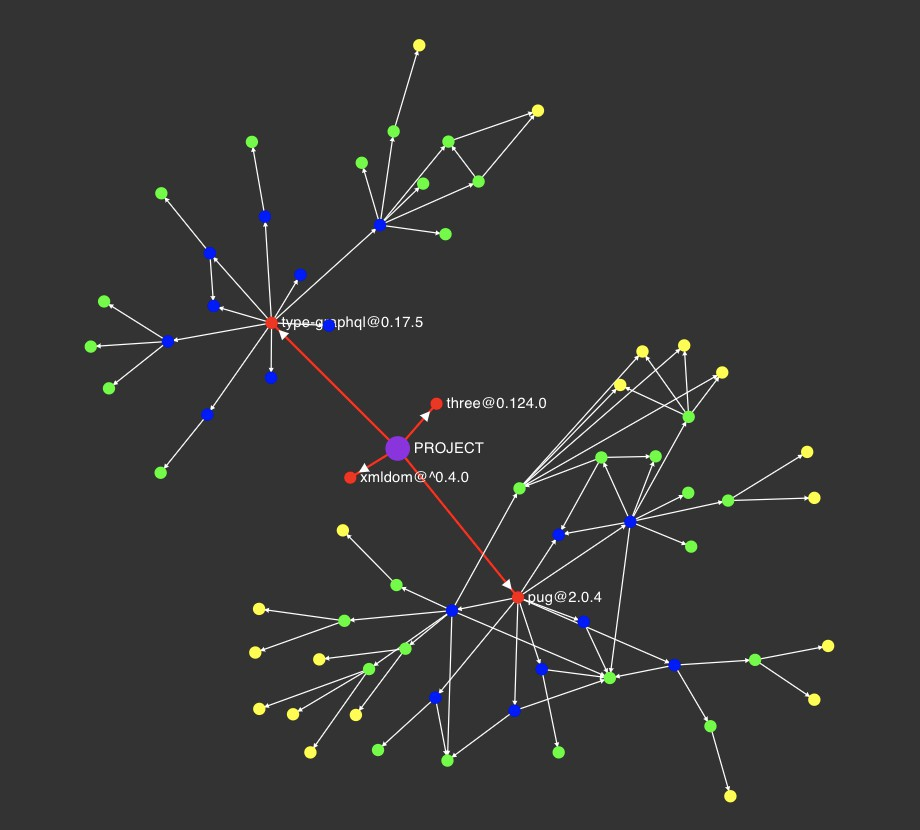
\includegraphics[width=\columnwidth]{Figures/Achilles-Test1.jpeg}
		\caption{Dependency graph visualization of Task 1}
		\label{fig:graphtest1}
	\end{figure}
	
	
	\begin{table}[tb]
		\centering
		\caption{Task 2: Vulnerabilities with Indirect Dependencies}
		\begin{tabular}{llcccc}
			\toprule
			No & Dependency & Version & Severity & Type & Category \\
			\midrule
			1 & netmask & 2.0.0 & High & Direct & HD \\ 
			2 & base64-url & 1.2.1 & High & Indirect & HI \\
			3 & angular-expressions & 1.1.1 & Low & Direct & LD \\ 
			4 & minimist & 1.2.0 & Low & Indirect & LI \\
			\bottomrule
		\end{tabular}
		\label{table:cha-test2}
	\end{table}
	
	\begin{figure}[tb]
		\centering
		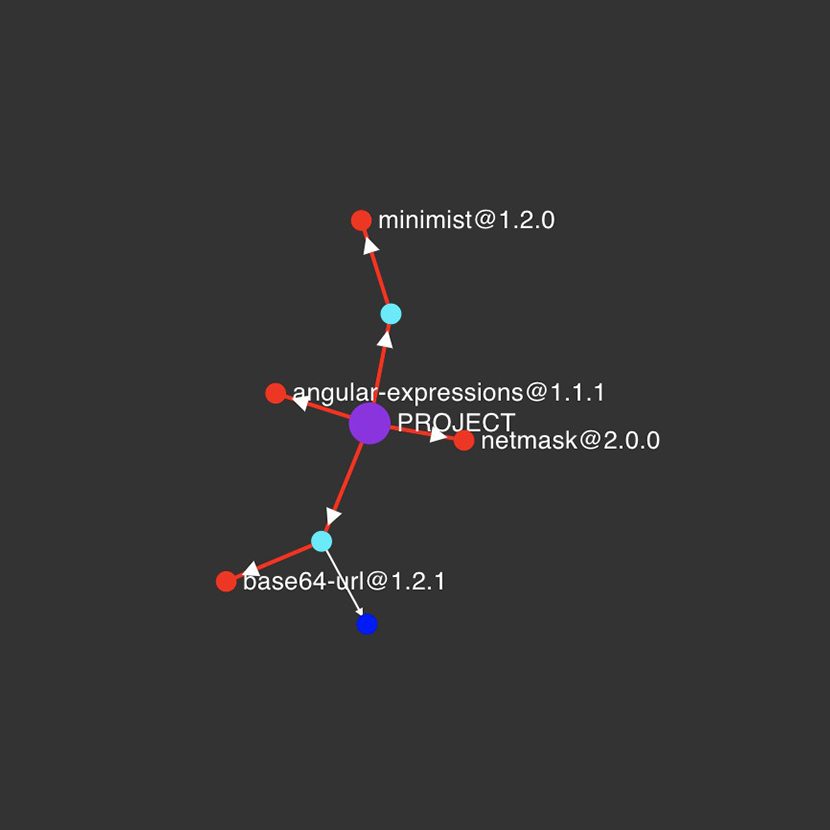
\includegraphics[width=0.8\columnwidth]{Figures/Achilles-Test2.png}
		\caption{Dependency graph visualization of Task 2}
		\label{fig:graphtest2}
	\end{figure}
	
	For Task 2, we aim to test whether the dependency graph visualization which shows the types of the vulnerabilities (direct or indirect) would affect the participants’ decision on dependency prioritization. We also created an npm project for this task and also made sure they could be detected by the 3 tools. The selected 4 dependencies include \texttt{netmask}, \texttt{base64-url}, \texttt{angular-expressions}, and \texttt{minimist}. Two dependencies, \texttt{netmask} and \texttt{base64-url}, had high severity vulnerabilities, while \texttt{angular-expressions} and \texttt{minimist} had low severity vulnerabilities. Table \ref{table:cha-test2} and Figure \ref{fig:graphtest2} shows the information of dependencies in Task 2 and how they depended on each other respectively. We can see from the visualization that \texttt{angular-expressions} and \texttt{netmask} are the direct dependency of the project, while \texttt{minimist} and \texttt{base64-url} are indirect dependencies of the project.
	
	\subsubsection{Outcome measurements} We compared the prioritization results and the prioritizing factors that the participants used before (i.e., based on the security vulnerability report from Dependabot) and after (i.e., based on the security vulnerability report from npm audit or \texttt{Achilles}) of the two tasks.  %We also compared the results between different types of visualization which are table by npm audit and graph by Achilles.
	
	%\subsubsection{Debrief} - We told the participants about the purpose of this experiment and interview them for them about the criteria that they used and the tool feedback.
	
	% \section{Participants’ demographic data
	
	\section{Results and Discussion}
	This section describes the results and discusses key observations from the user study.
	
	\subsection{Task 1: Vulnerabilities with Complex Dependencies}
	
	%Task 1 contains 4 direct dependencies with different levels of severity and complexity (the number of other dependencies that the dependencies in the project are relied on). The participants of both the controlled group and experimental group were given the same project with the same dependencies. We discuss their results below.
	The result from performing Task 1 is discussed below.
	
	\subsubsection{Experimental Group (\texttt{Achilles})}
	According to Table \ref{table:result-Ach-t1}, we found two sub groups of participants according to the prioritization order. We call them \textit{changed group} and \textit{unchanged group}. The changed group contains the participants who the dependency prioritization after seeing \texttt{Achilles} report differ from the  initial prioritization based on Dependabot report, i.e., they changed their ranking of the vulnerable dependencies to be fixed. The unchanged group contains the participants who the dependency prioritization were the same between \texttt{Achilles} and Dependabot.
	
	The changed group includes 7 participants (A1, A2, A4, A5, A7, A8, and A9). We observed that they only emphasized on severity when they saw the vulnerability report from Dependabot. However, after they used \texttt{Achilles}, they also took other factors into account. Within the changed group, six participants (A1, A2, A4, A5, A7, and A8) took \textit{the dependency's complexity} into account. 
	%However, A9 was only concerned about the severity more after using Achilles, and the participant mentioned that the package's complexity did not have influence on the prioritization.
	%Within the six participants in the changed group, three participants (A1, A4, A5) used severity as the first priority factor and high complexity as the second priority factor. On the other hand, one participant (A7) used low complexity as the second priority factor. For two participants who use complexity as the first priority factor and high severity as the second priority factor, A2 prioritized high complexity first, while A8 prioritized low complexity first.
	
	The unchanged group (A3, A6, and A10) does not change their prioritization order. Nonetheless, they all mentioned that after they see \texttt{Achilles}, they get information about the package's complexity easier.
	
	According to Table \ref{table:prioritization_factor}, after seeing the vulnerability report from Dependabot, seven participants use severity as the significant factor for the prioritization. After using the dependency graph visualization in \texttt{Achilles}, there are six cases where the package complexity has become one of the factors when prioritizing the package update, either as the first or the second priority factor.
	
	\begin{table*}
		\caption{Task 1 Vulnerabilities with Complexities: Result by Participants}
		\centering
		\begin{tabular}{clll|clll}
			\toprule
			\multicolumn{4}{c|}{Experimental Group} & \multicolumn{4}{c}{Controlled Group}  \\ 
			\midrule
			Participants         & Tool       & Dependency Prioritization & Comparison & Participants & Tool  & Dependency Prioritization & Comparison \\ 
			\midrule
			\multirow{2}{*}{A1}   & Dependabot    & HC \textgreater{}= HS \textgreater LC \textgreater{}= LS & \multirow{2}{*}{Different} & \multirow{2}{*}{N1} & Dependabot & HS \textgreater HC \textgreater LS \textgreater LC & \multirow{2}{*}{Same} \\ 
			& \texttt{Achilles}      & HC \textgreater HS \textgreater LC \textgreater LS       & & & npm audit & HS \textgreater HC \textgreater LS \textgreater LC & \\ \midrule
			\multirow{2}{*}{A2}   & Dependabot    & HS \textgreater{}= HC \textgreater LC \textgreater LS    & \multirow{2}{*}{Different} & \multirow{2}{*}{N2} & Dependabot & HC \textgreater HS \textgreater LC \textgreater LS & \multirow{2}{*}{Different} \\ 
			& \texttt{Achilles}      & HC \textgreater LC \textgreater HS \textgreater LS       & & & npm audit & HC \textgreater HS \textgreater LC \textgreater{}= LS & \\ \midrule
			\multirow{2}{*}{A3}   & Dependabot    & HS \textgreater{}= HC \textgreater LC \textgreater{}= LS & \multirow{2}{*}{Same} & \multirow{2}{*}{N3} & Dependabot & HC \textgreater HS \textgreater LC \textgreater{}= LS & \multirow{2}{*}{Same} \\ 
			& \texttt{Achilles}      & HS \textgreater{}= HC \textgreater LC \textgreater{}= LS & & & npm audit & HC \textgreater HS \textgreater LC \textgreater{}= LS & \\ \midrule
			\multirow{2}{*}{A4}   & Dependabot    & HS \textgreater{}= HC \textgreater LC \textgreater{}= LS & \multirow{2}{*}{Different} & \multirow{2}{*}{N4} & Dependabot & HS \textgreater HC \textgreater LC \textgreater{}= LS  & \multirow{2}{*}{Different} \\ 
			& \texttt{Achilles}      & HC \textgreater HS \textgreater LC \textgreater LS       & & & npm audit & HC \textgreater HS \textgreater LS \textgreater LC & \\ \midrule
			\multirow{2}{*}{A5}   & Dependabot    & HC \textgreater HS \textgreater LS \textgreater LC       & \multirow{2}{*}{Different} & \multirow{2}{*}{N5} & Dependabot & HS \textgreater HC \textgreater LC \textgreater LS & \multirow{2}{*}{Same} \\ 
			& \texttt{Achilles}      & HS \textgreater HC \textgreater LS \textgreater LC       & & & npm audit & HS \textgreater HC \textgreater LC \textgreater LS & \\ \midrule
			\multirow{2}{*}{A6}   & Dependabot    & HC \textgreater{}= HS \textgreater LC \textgreater{}= LS & \multirow{2}{*}{Same} & \multirow{2}{*}{N6} & Dependabot & HS \textgreater{}= HC \textgreater LS \textgreater{}= LC & \multirow{2}{*}{Same} \\ 
			& \texttt{Achilles}      & HC \textgreater{}= HS \textgreater LC \textgreater{}= LS & & & npm audit & HS \textgreater{}= HC \textgreater LS \textgreater{}= LC & \\ \midrule
			\multirow{2}{*}{A7}   & Dependabot    & LS \textgreater LC \textgreater HS \textgreater HC       & \multirow{2}{*}{Different} & \multirow{2}{*}{N7} & Dependabot & LC \textgreater HS \textgreater LS \textgreater HC& \multirow{2}{*}{Same} \\ 
			& \texttt{Achilles}      & HS \textgreater{}= LS \textgreater HC \textgreater LC    & & & npm audit & LC \textgreater HS \textgreater LS \textgreater HC& \\ \midrule
			\multirow{2}{*}{A8}   & Dependabot    & HS \textgreater HC \textgreater LC \textgreater LS       & \multirow{2}{*}{Different} & \multirow{2}{*}{N8}  & Dependabot & HC \textgreater HS \textgreater LS \textgreater LC & \multirow{2}{*}{Different} \\ 
			& \texttt{Achilles}      & HS \textgreater{}= LS \textgreater HC \textgreater LC    & & & npm audit & HS \textgreater HC \textgreater LC \textgreater{}= LS & \\ \midrule
			\multirow{2}{*}{A9}   & Dependabot    & HS \textgreater LC \textgreater LS \textgreater HC       & \multirow{2}{*}{Different} & \multirow{2}{*}{N9} & Dependabot & HS \textgreater{}= HC \textgreater{}= LC \textgreater LS  & \multirow{2}{*}{Different} \\ 
			& \texttt{Achilles}      & HS \textgreater HC \textgreater LC \textgreater LS       & & & npm audit & HS \textgreater{}= HC \textgreater{}= LC \textgreater{}= LS & \\ \midrule
			\multirow{2}{*}{A10}  & Dependabot    & HC \textgreater{}= HS \textgreater LC \textgreater{}= LS & \multirow{2}{*}{Same} & \multirow{2}{*}{N10} & Dependabot & HC \textgreater{}= HS \textgreater LC \textgreater{}= LS & \multirow{2}{*}{Same} \\ 
			& \texttt{Achilles}      & HS \textgreater{}= HC \textgreater LC \textgreater{}= LS & & & npm audit & HC \textgreater{}= HS \textgreater LC \textgreater{}= LS & \\ \midrule
			\multicolumn{8}{l}{H = High severity, L = Low severity, C = Complex (has several dependencies), S = Simple (no dependency)} \\
		\end{tabular}
		\label{table:result-Ach-t1}
	\end{table*}
	
	\begin{table}[tb]
		\caption{Factors for Prioritizing Dependency Fixes}
		\centering
		\resizebox{0.49\textwidth}{!}{%
			\begin{tabular}{cp{2cm}p{2cm}p{1.5cm}r} 
				\toprule
				Tool & First factor & Second factor & Participants & Amount \\ 
				\midrule
				\multicolumn{5}{l}{\textit{Task 1 Complexity}}  \\
				\midrule
				\multirow{7}{*}{Dependabot} & High Severity & Low Severity & A1, A2, A3, A4, A5, A6, A10  & 7  \\ 
				& High Severity & Recent use  & A8 & 1 \\ 
				& Version No. & - & A9 & 1 \\ 
				& Indirect dep. & - & A7 & 1  \\ 
				\midrule
				\multirow{6}{*}{\texttt{Achilles}}  & High Severity & Low Severity                    & A3, A6, A10                                                            & 3               \\ 
				&  High Severity & High Complexity                 & A1, A4, A5                                                             & 3               \\ 
				&  High Severity & Low Complexity                  & A7                                                                     & 1               \\ 
				&  High Severity  & Version                         & A9                                                                     & 1               \\ 
				& High Complexity                         & High Severity                   & A2                                                                     & 1               \\ 
				& Low Complexity                          & High Severity                   & A8                                                                     & 1               \\ 
				\midrule
				\multicolumn{5}{l}{\textit{Task 2 Direct/Indirect Dependency}}  \\
				\midrule
				\multirow{7}{*}{Dependabot} & High Severity  & Low Severity                    & A1, A2, A4, A10                                & 4               \\ 
				& High Severity & Direct dep.                         & A5                                            & 1               \\ 
				& High Severity & Issue type                      & A6                                            & 1               \\ 
				& High Severity & Recent use                      & A8                                            & 1               \\ 
				& Direct dep.  & High Severity                   & A3                                            & 1               \\ 
				& Indirect dep. & Severity                        & A9                                            & 1               \\ 
				& Indirect dep. & - & A7                                            & 1               \\ 
				\midrule
				\multirow{5}{*}{\texttt{Achilles}}  & High Severity & Direct dep.                          & A1, A5, A6, A8, A10                           & 5               \\ 
				& Direct dep.  & High Severity                   & A2, A3, A4 & 3               \\ 
				& High Severity & Version                         & A9                                            & 1               \\ 
				& Indirect dep. & Severity                        & A7                                            & 1               \\ 
				\bottomrule
			\end{tabular}
		}
		\label{table:prioritization_factor}
	\end{table}
	
	\subsubsection{Controlled Group (npm-audit)}
	According to Table \ref{table:result-Ach-t1}, we similarly found two sub groups of participants, changed and unchanged groups, according to the prioritization order.
	
	There are four participants in the changed group, including N2, N4, N8, and N9. They shift the prioritization order after using npm audit. Even though there is no significant change in the prioritization order, the report from Dependabot and npm audit provide vulnerability information at different granularity. It affects the prioritization order since these participants use vulnerability information (CVE) as the prioritization criteria. Six participants in the unchanged group gave the same dependency prioritization between Dependabot and npm audit.
	
	%On the other hand, there are six participants (N1, N3, N5, N6, N7 and N10) in the unchanged group. Five of them (N1, N3, N5, N6 N10) use severity as the top priority factor for both tools' prioritization. Participant N7 uses the ease of patching the packages as the main priority factor for both tools.
	%According to Table \ref{table:audit-pri1}, 
	After using both Dependabot and npm audit, nine participants still used severity as the first priority factor.
	
	\subsection{Task 2: Vulnerabilities with Indirect Dependencies}
	Task 2 contains both direct and indirect vulnerabilities with different levels of severity. Similar to Task 1, the participants of both the controlled and experimental groups see the same project with the same dependencies. We discuss their results below.
	
	\subsubsection{Experimental Group (\texttt{Achilles})}
	According to table \ref{table:ach-indirect},
	%there are two groups of participants categorized by the prioritization order.
	the changed group, including seven participants A1, A2, A4, A6, A7, A8, and A10, changed the prioritization order after seeing \texttt{Achilles} visualization.  	
	The unchanged group (A3, A5, A9) did not change their prioritization order. Participant A3 choose to update direct dependencies first since seeing the vulnerabilities report from Dependabot. Participant A5 updates the high severity vulnerabilities first and takes direct dependencies into account since seeing the report, but without changing the prioritization. Participant A9 considers the severity level and the version number. Nevertheless, they mentioned that \texttt{Achilles} allows them to differentiate between direct and indirect vulnerabilities easier, similarly to Task 1.
	
	From Table~\ref{table:prioritization_factor}, based on the vulnerability report from Dependabot, participants A1, A2, A4, and A10 only emphasized on severity of the vulnerable packages. Participant A6 also considered issue type. Participant A8 takes recency of the vulnerability into account. However, participant A10 did not concern about the severity, only the number of indirect dependencies.
	
	Nonetheless, after using \texttt{Achilles}, many participants took the types of dependency (whether directly or indirectly) into account. Within the changed group, four participants A1, A6, A8, and A10, use severity as their first priority factor and for the second priority factor, consider updating direct dependencies first. Two participants, A2 and A4, choose to update direct dependencies first and select high severity as the second priority factor. On the other hand, participant A7 updates the indirect dependencies first before considering the severity level.
	
	
	
	\begin{table*}[tb]
		\caption{Task 2 Vulnerabilities with Direct/Indirect Dependencies: Result by Participants}
		\centering
		\begin{tabular}{clll|clll}
			\toprule
			\multicolumn{4}{c|}{Experimental Group} & \multicolumn{4}{c}{Controlled Group}  \\ 
			\midrule
			Participants         & Tool       & Dependency Prioritization & Comparison & Participants & Tool  & Dependency Prioritization & Comparison \\ 
			\midrule
			\multirow{2}{*}{A1}  & Dependabot & HD \textgreater{}= HI \textgreater LI \textgreater{}= LD    & \multirow{2}{*}{Different}      & \multirow{2}{*}{N1} & Dependabot & HD \textgreater LD \textgreater HI \textgreater LI  & \multirow{2}{*}{Same} \\ 
			& \texttt{Achilles}   & HD \textgreater HI \textgreater LD \textgreater LI & & & npm audit & HD \textgreater LD \textgreater HI \textgreater LI & \\ 
			\midrule
			\multirow{2}{*}{A2}  & Dependabot & HD \textgreater{}= HI \textgreater{}= LI \textgreater{}= LD & \multirow{2}{*}{Different}      & \multirow{2}{*}{N2} & Dependabot & HD\textgreater HI \textgreater LI \textgreater = LD &  \multirow{2}{*}{Same} \\
			& \texttt{Achilles}   & HD \textgreater LD \textgreater LI \textgreater HI & & & npm audit & HD\textgreater HI \textgreater LI \textgreater = LD &  \\ 
			\midrule
			\multirow{2}{*}{A3}  & Dependabot & HD \textgreater LD \textgreater HI \textgreater{}= LI & \multirow{2}{*}{Same} & \multirow{2}{*}{N3} & Dependabot & HI \textgreater{}= HD \textgreater LD \textgreater{}= LI &  \multirow{2}{*}{Different} \\ 
			& \texttt{Achilles}   & HD \textgreater LD \textgreater HI \textgreater{}= LI & & & npm audit & HD \textgreater LD \textgreater HI \textgreater LI  & \\ 
			\midrule
			\multirow{2}{*}{A4}  & Dependabot & HD \textgreater{}= HI \textgreater LI \textgreater{}= LD    & \multirow{2}{*}{Different}      & \multirow{2}{*}{N4} & Dependabot & HD \textgreater HI \textgreater LI \textgreater LD & \multirow{2}{*}{Different} \\ 
			& \texttt{Achilles}   & HD \textgreater LD \textgreater HI \textgreater LI & & & npm audit &  HD \textgreater LD \textgreater HI \textgreater LI & \\ 
			\midrule
			\multirow{2}{*}{A5}  & Dependabot & HD \textgreater HI \textgreater LD \textgreater LI          & \multirow{2}{*}{Same}           & \multirow{2}{*}{N5} & Dependabot & HD \textgreater{}= HI \textgreater LD \textgreater{}= LI & \multirow{2}{*}{Same} \\ 
			& \texttt{Achilles}   & HD \textgreater HI \textgreater LD \textgreater LI & & & npm audit & HD \textgreater{}= HI \textgreater LD \textgreater{}= LI  & \\ 
			\midrule
			\multirow{2}{*}{A6}  & Dependabot & HD \textgreater{}= HI \textgreater LD \textgreater LI       & \multirow{2}{*}{Different}      & \multirow{2}{*}{N6} & Dependabot & HD \textgreater{}= HI \textgreater LI \textgreater{}= LD & \multirow{2}{*}{Different} \\ 
			& \texttt{Achilles}   & HD \textgreater HI \textgreater LD \textgreater LI & & & npm audit & HD \textgreater LD \textgreater HI \textgreater LI & \\ 
			\midrule
			\multirow{2}{*}{A7}  & Dependabot & HD \textgreater HI \textgreater LD \textgreater LI & \multirow{2}{*}{Different}      & \multirow{2}{*}{N7} & Dependabot & HD \textgreater LD \textgreater{}= LI \textgreater HI & \multirow{2}{*}{Different} \\  
			& \texttt{Achilles}   & HD \textgreater LD \textgreater LI \textgreater HI & & & npm audit & HD \textgreater LD \textgreater LI \textgreater HI &  \\ 
			\midrule
			\multirow{2}{*}{A8}  & Dependabot & HD \textgreater HI \textgreater LI \textgreater{}= LD       & \multirow{2}{*}{Different}      & \multirow{2}{*}{N8} & Dependabot & HD \textgreater LI \textgreater{}= LD \textgreater HI & \multirow{2}{*}{Different} \\ 
			& \texttt{Achilles}   & HD \textgreater{}= HI \textgreater LI \textgreater{}= LD    &                                 & & npm audit & HD \textgreater HI \textgreater LI \textgreater{}= LD & \\ 
			\midrule
			\multirow{2}{*}{A9}  & Dependabot & LI \textgreater{}= LD \textgreater{}= HI \textgreater{}= HD & \multirow{2}{*}{Same}           & \multirow{2}{*}{N9} & Dependabot & HD \textgreater{}= HI \textgreater{}= LI \textgreater{}= LD & \multirow{2}{*}{Different} \\ 
			& \texttt{Achilles}   & HI \textgreater{}= HD \textgreater{}= LI \textgreater{}= LD &                                 & & npm audit & HI \textgreater{}= HD \textgreater LI \textgreater{}= LD &  \\ 
			\midrule
			\multirow{2}{*}{A10} & Dependabot & HD \textgreater{}= HI \textgreater LI \textgreater{}= LD    & \multirow{2}{*}{Different}      & \multirow{2}{*}{N10} & Dependabot & HD \textgreater HI \textgreater LD \textgreater LI & \multirow{2}{*}{Same} \\ 
			& \texttt{Achilles}   & HD \textgreater LD \textgreater HI \textgreater LI          &                                 & & npm audit & HD \textgreater HI \textgreater LD \textgreater LI & \\ 
			\bottomrule
			\multicolumn{8}{l}{H = High severity, L = Low severity, D = Direct dependency, I = Indirect dependency} \\
		\end{tabular}
		\label{table:ach-indirect}
	\end{table*}
	
	%	\begin{table*}[tb]
	%		\caption{Factors for Prioritizing Package Updates}
	%		\centering
	%		\begin{tabular}{|c|c|c|c|c|}
	%			\hline
	%			\textbf{Tool} & \textbf{First priority factor}  & \textbf{Second priority factor} & \textbf{Cases}                                & \textbf{Number} \\ \hline
	%			\multicolumn{1}{|c|}{\multirow{8}{*}{\textbf{Dependabot}}} & \multirow{4}{*}{High Severity}  & Low Severity                    & A1,A2, A4, A10                                & 4               \\ \cline{3-5} 
	%			\multicolumn{1}{|c|}{}                                     &                                 & Direct                          & A5                                            & 1               \\ \cline{3-5} 
	%			\multicolumn{1}{|c|}{}                                     &                                 & Issue type                      & A6                                            & 1               \\ \cline{3-5} 
	%			\multicolumn{1}{|c|}{}                                     &                                 & Recent use                      & A8                                            & 1               \\ \cline{2-5} 
	%			\multicolumn{1}{|c|}{}                                     & Direct                          & High Severity                   & A3                                            & 1               \\ \cline{2-5} 
	%			\multicolumn{1}{|c|}{}                                     & Indirect                        & Severity                        & A9                                            & 1               \\ \cline{2-5} 
	%			\multicolumn{1}{|c|}{}                                     & Number of indirect dependencies & \multicolumn{1}{l|}{}           & A7                                            & 1               \\ \cline{2-5} 
	%			\multicolumn{1}{|c|}{}                                     & \multicolumn{3}{c|}{\textbf{Total}}                                                                               & 10              \\ \hline
	%			\multicolumn{1}{|c|}{\multirow{5}{*}{\textbf{Achilles}}}   & \multirow{2}{*}{High Severity}  & Direct                          & A1, A5, A6, A8, A10                           & 5               \\ \cline{3-5} 
	%			\multicolumn{1}{|c|}{}                                     &                                 & Version                         & A9                                            & 1               \\ \cline{2-5} 
	%			\multicolumn{1}{|c|}{}                                     & Direct                          & High Severity                   & A2(with third factor of low severity), A3, A4 & 3               \\ \cline{2-5} 
	%			\multicolumn{1}{|c|}{}                                     & Indirect                        & Severity                        & A7                                            & 1               \\ \cline{2-5} 
	%			\multicolumn{1}{|c|}{}                                     & \multicolumn{3}{c|}{\textbf{Total}}                                                                               & 10              \\ \hline
	%		\end{tabular}
	%		\label{table:ach-pri-indirect}
	%	\end{table*}
	
	%After seeing the graph visualization in Achilles, there are seven participants whose types of dependency have become the factor when they are prioritizing the package update as the first or the second priority factor. 
	
	\subsubsection{Controlled Group (npm-audit)}
	%	According to table \ref{table:ach-indirect}, there are two groups of participants categorized by the prioritization order.
	According to Table~\ref{table:ach-indirect}, six participants are in the changed group (N3, N4, N6, N7, N8 and N9) and four participants are in the unchanged group (N1, N2, N5, and N10). 
	
	%Even though participant N1 did not change the order, the criteria is different. After seeing Dependabot report, participant N1 uses existing solving pull request and severity as the factor, and after seeing the npm audit report, the participant considers direct dependency and severity. Participants N2, N5, and N9 only assess the severity.
	
	When they saw the vulnerability report from Dependabot, they prioritized severity as the first or second factor. Participants N3 and N6 used severity as their only factors. Participant N4 also considerd the CVE, and participant N7 prioritized the ease of fixing. Participant N8 only took vulnerabilities information into account. Participant N10 considered the risk of vulnerabilities from attacker. However, after they used npm audit, participants N3 and N6 considered the types of vulnerabilities as a factor for prioritization. N4, N7 and N8 mentioned that short description that is provided by npm affected their decision on the prioritization. Participant N10 only considered the severity.
	
	%According to Table \ref{table:npm-pri2}, after seeing the vulnerability report from Dependabot, eight participants use severity as the major factor for prioritization. After seeing the graph visualization in \texttt{Achilles}, there are four participants whose types of dependency have become the factor when they prioritize the package update as the first or second priority factor.
	
	\subsection{Answers to Research Questions}
	From the results, we can answer the two research questions as follows.
	
	\subsubsection{RQ1: How well does the dependency graph visualization support developer’s decision on prioritizing vulnerability to fix?}
	From the user study, six participants take complexity into account after seeing the graph visualization. Nine out of ten participants consider types of dependencies (direct or indirect dependencies) as the factor for prioritization after seeing the graph visualization.
	To answer the RQ, \textbf{we found that the graph visualization of \texttt{Achilles} helps supporting developers' decisions on prioritizing vulnerability to fix by providing more information about complexity and direct/indirect dependencies compared to the traditional list of vulnerabilities provided by Dependabot}.
	
	\subsubsection{RQ2: How well does the dependency graph visualization perform compared to the state-of-the-art tools?}
	
	We found some differences between our dependency graph visualization and state-of-the-art tools on affecting developers' decision on prioritizing vulnerabilities to fix. 
	
	We can see from Table~\ref{table:result-Ach-t1}, in Task 1 where vulnerable packages have different complexities, the number of participants who used \texttt{Achilles} and changed their prioritization order is larger than the number of participants who used npm audit. The list of vulnerabilities provided by npm audit affected the developers' decision 4 out of 10 cases, while the dependency graph visualization affected the developers' decision to update vulnerabilities 7 out of 10 cases. %Table \ref{table:compare-ach} Comparison of developers' decisions after seeing the graph and table visualization on the task with indirect vulnerabilities
	
	%Table \ref{table:compare-ach} Comparison of developers' decisions after seeing the graph and table visualization on the task having vulnerabilities with complexity
	
	\begin{table}[tb]
		\centering
		\caption{Comparison of Developers' Decisions Using the Tools Compared to Dependabot Report}
		\begin{tabular}{llrr}
			\toprule
			Task & Decision & \texttt{Achilles} & npm audit \\
			\midrule
			\multirow{2}{*}{Task 1} & Same & 3 & 6 \\ 
			& Different & 7 & 4 \\ \midrule
			\multirow{2}{*}{Task 2} & Same & 3 & 4 \\ 
			& Different & 7 & 6 \\
			\bottomrule
		\end{tabular}
		\label{table:compare-ach}
	\end{table}
	
	We can see from Table~\ref{table:ach-indirect}, for Task 2 where vulnerable packages have different types of dependencies. The number of participants who use \texttt{Achilles} and change the prioritization order is also larger than participants who use npm audit. The graph visualization in \texttt{Achilles} does outperform npm audit in providing information about the types of dependencies since both of the tools represent direct and indirect dependencies differently. However, the differences between the two group is not as large as in Task 1. The list of vulnerabilities provided by npm audit affected the developers' decision 6 out of 10 cases, while the dependency graph visualization affected the developers' decision to update vulnerabilities 7 out of 10 cases.
	
	The result of asking the participants who used npm audit to see \texttt{Achilles} visualization of Task 1 and Task 2 and performed the prioritization again is shown in Table \ref{table:x3}. In Task 1, there are seven participants change their prioritization since they consider complexity of the packages which introduced by \texttt{Achilles} as a prioritization factor. There is no significant differences in Task 2 since both \texttt{Achilles} and npm audit provide types of dependencies (whether direct or indirect dependencies).
	
	To answer the RQ, \textbf{the dependency graph visualization offers more information to the developers and supports their decision on prioritization of the dependencies to fix better than npm audit.} We found large differences of dependency prioritization between \texttt{Achilles} and npm audit when the project contains dependencies with complexities. However, in the case of the project containing direct/indirect dependencies, the differences between the two tools are small.
	
	\begin{table}[tb]
		\centering
		\caption{Developers' Decisions using \texttt{Achilles} Compared to npm audit}
		\begin{tabular}{ccc} 
			\toprule
			Decision & Task 1 & Task 2 \\
			\midrule
			Same & 3 & 5\\ 
			Different & 7 & 5 \\
			\bottomrule
		\end{tabular}
		\label{table:x3}
	\end{table}

	\section{Threats to Validity}
	\textbf{Internal validity:} We recruited 20 participants for our user study with the inclusion criteria that the participants must have programming experience of at least six months and have fundamental knowledge in software vulnerabilities and related tools. However, there is a possibility that some of the participants may not be familiar with Dependabot or npm audit. This may affect the result of the user study because the participants may not compare the tools with their full understandings. We mitigate this threat by providing two example tasks for them to train and understand how the tools work before performing the actual study. 
	
	\textbf{External validity:} We simulate the actual dependency prioritization activity by creating the two tasks used in the user study. Thus, the prioritization results the factors for prioritization may be limited to only such scenarios and vulnerabilities captured by the two tasks and may not be generalized to all the cases of npm security vulnerabilities.
	
	\section{Conclusion}
	Using third-party dependencies is a common activity in modern software development. Dependency adoption can speed up the development but, at the same time, can also come with a cost. Direct and indirect dependencies included in a software project may be vulnerable and they introduce weaknesses into the software. Security vulnerabilities in software dependencies are difficult to detect because the need of relevant and timely information of the dependencies used in the project. Moreover, the complexity of dependency relationships within a project makes the prioritization of the vulnerable dependencies to be updated a challenging task. 
	
	In this work, we present a visualization of npm project dependencies using dependency graph to help the developers prioritize a vulnerable dependency update. We create a web-based interactive tool called \texttt{Achilles} that analyzes GitHub projects and creates a dependency graph to show direct and indirect dependencies and their vulnerabilities. By using force-directed graph, \texttt{Achilles}s allows the developers to explore dependencies in their software intuitively and, at the same time, provides additional information for the vulnerable dependencies to help the developers to make decision on updating such dependencies. 
	
	We performed a user study with 20 participants to evaluate how \texttt{Achilles} helps the developers to change their dependency prioritization based on the vulnerability report by Dependabot. The results show that 7 out of the 10 participants who used \texttt{Achilles} after Dependabot changed their prioritization in the two tasks given to them. This is due to the additional information provided by \texttt{Achilles} including complexity and indirect dependencies. On the other hand, only 4 out of 10 participants who used npm audit after Dependabot changed their prioritization in Task 1 and 6 out of 10 participants changed their prioritization in Task 2. 
	
	Our work shows that dependency graph can be an effective visualization that help npm developers understand their software project better and also make better decisions on security fixes and prioritizing dependency updates.
	
	%There are several dependency managers that manage the installation of the third-party dependencies. For JavaScript, npm is a dependency manager for Node.js and is widely used among the developers. 
	
	\bibliographystyle{IEEEtranN}
	\bibliography{references.bib}
	
	% BACKUP %
%	\clearpage
%	
%	\section{These are backup data}
%	
%	\begin{table*}[tb]
%		\centering
%		\caption{The Result of npm audit Task Case No. 1 (Complexity)}
%		\begin{tabular}{|l|l|l|c|l|l|}
%			\hline
%			Participants         & Tool       & Answers                                                     & \multicolumn{1}{l|}{Comparison} & First Priority                    & Second Priority            \\ \hline
%			\multirow{3}{*}{N1}  & Dependabot & HS \textgreater HC \textgreater LS \textgreater LC          & \multirow{2}{*}{Same}           & High severity                     & Alerted Time               \\ \cline{2-3} \cline{5-6} 
%			& npm-audit  & HS \textgreater HC \textgreater LS \textgreater LC          &                                 & High severity                     & -                          \\ \cline{2-6} 
%			& Achilles   & HS \textgreater{}= LS \textgreater HC \textgreater{}= LC    & different                       &                                   &                            \\ \hline
%			\multirow{3}{*}{N2}  & Dependabot & HC \textgreater HS \textgreater LC \textgreater LS          & \multirow{2}{*}{Different}      & Severity                          & Impact on the server?      \\ \cline{2-3} \cline{5-6} 
%			& npm-audit  & HC \textgreater HS \textgreater LC \textgreater{}= LS       &                                 & High severity                     &                            \\ \cline{2-6} 
%			& Achilles   & HS \textgreater HC \textgreater LS \textgreater LC          & Different                       & Severity                          & Less complex               \\ \hline
%			\multirow{3}{*}{N3}  & Dependabot & HC \textgreater HS \textgreater LC \textgreater{}= LS       & \multirow{2}{*}{Same}           & High severity                     & Impact with the project    \\ \cline{2-3} \cline{5-6} 
%			& npm-audit  & HC \textgreater HS \textgreater LC \textgreater{}= LS       &                                 &                                   &                            \\ \cline{2-6} 
%			& Achilles   & HS \textgreater HC \textgreater LS \textgreater LC          & Different                       & High severity                     & Low complexity             \\ \hline
%			\multirow{3}{*}{N4}  & Dependabot & HS \textgreater HC \textgreater LC \textgreater{}= LS       & \multirow{2}{*}{Different}      & High severity                     & CVE                        \\ \cline{2-3} \cline{5-6} 
%			& npm-audit  & HC \textgreater HS \textgreater LS \textgreater LC          &                                 & High severity                     & npm description            \\ \cline{2-6} 
%			& Achilles   & HC \textgreater HS \textgreater LS \textgreater LC          & Same                            & High seveirty                     & newer CVE                  \\ \hline
%			\multirow{3}{*}{N5}  & Dependabot & HS \textgreater HC \textgreater LC \textgreater LS          & \multirow{2}{*}{Same}           & High severity                     &                            \\ \cline{2-3} \cline{5-6} 
%			& npm-audit  & HS \textgreater HC \textgreater LC \textgreater LS          &                                 & High severity                     &                            \\ \cline{2-6} 
%			& Achilles   & HS \textgreater HC \textgreater LS \textgreater LC          & Different                       & High severity                     & Less indirect dependencies \\ \hline
%			\multirow{3}{*}{N6}  & Dependabot & HS \textgreater{}= HC \textgreater LS \textgreater{}= LC    & \multirow{2}{*}{Same}           & High severity                     &                            \\ \cline{2-3} \cline{5-6} 
%			& npm-audit  & HS \textgreater{}= HC \textgreater LS \textgreater{}= LC    &                                 & High severity                     &                            \\ \cline{2-6} 
%			& Achilles   & HS \textgreater LS \textgreater HC \textgreater LC          & Different                       & Less indirect dependencies        & Severity                   \\ \hline
%			\multirow{3}{*}{N7}  & Dependabot & LC \textgreater HS \textgreater LS \textgreater HC          & \multirow{3}{*}{Same}           & The ease of patching the packages &                            \\ \cline{2-3} \cline{5-6} 
%			& npm-audit  & LC \textgreater HS \textgreater LS \textgreater HC          &                                 & The ease of patching the packages &                            \\ \cline{2-3} \cline{5-6} 
%			& Achilles   & LC \textgreater HS \textgreater LS \textgreater HC          &                                 & The ease of patching the packages &                            \\ \hline
%			\multirow{3}{*}{N8}  & Dependabot & HC \textgreater HS \textgreater LS \textgreater LC          & \multirow{3}{*}{Different}      & Severity                          & Vulnerability risk         \\ \cline{2-3} \cline{5-6} 
%			& npm-audit  & HS \textgreater HC \textgreater LC \textgreater{}= LS       &                                 & Severity                          & expected error             \\ \cline{2-3} \cline{5-6} 
%			& Achilles   & HC \textgreater HS \textgreater LC \textgreater LS          &                                 & High severity                     & More indirect dependencies \\ \hline
%			\multirow{3}{*}{N9}  & Dependabot & HS \textgreater{}= HC \textgreater{}= LC \textgreater LS    & \multirow{3}{*}{Same}           & High severity                     &                            \\ \cline{2-3} \cline{5-6} 
%			& npm-audit  & HS \textgreater{}= HC \textgreater{}= LC \textgreater{}= LS &                                 & High severity                     &                            \\ \cline{2-3} \cline{5-6} 
%			& Achilles   & HS \textgreater{}= HC \textgreater{}= LC \textgreater{}= LS &                                 & High severity                     &                            \\ \hline
%			\multirow{3}{*}{N10} & Dependabot & HC \textgreater{}= HS \textgreater LC \textgreater{}= LS    & \multirow{2}{*}{Same}           & High severity                     &                            \\ \cline{2-3} \cline{5-6} 
%			& npm-audit  & HC \textgreater{}= HS \textgreater LC \textgreater{}= LS    &                                 & High severity                     &                            \\ \cline{2-6} 
%			& Achilles   & HC \textgreater LC \textgreater HS \textgreater LS          & Different                       & Complexity                        & Severity                   \\ \hline
%			\multicolumn{5}{}{} H = High severity, L = Low severity, C = Complex (has several dependencies), S = Simple (no dependency) \\
%		\end{tabular}
%		\label{table:npm-comp}
%	\end{table*}
%	
%	\begin{table*}[tb]
%		\caption{Factors for Prioritizing Package Updates}
%		\begin{tabular}{|c|c|c|c|c|}
%			\hline
%			\multicolumn{1}{|l|}{}               & \textbf{First priority factor}     & \textbf{Second priority factor}          & \textbf{Cases}              & \textbf{Number} \\ \hline
%			\multirow{8}{*}{\textbf{Dependabot}} & \multirow{5}{*}{High Severity}     & Low Severity                             & N5, N6, N9, N10             & 4               \\ \cline{3-5} 
%			&                                    & Detail of vulnerability                  & N8                          & 1               \\ \cline{3-5} 
%			&                                    & Alert time                               & N1                          & 1               \\ \cline{3-5} 
%			&                                    & Impact with the project                  & N3                          & 1               \\ \cline{3-5} 
%			&                                    & CVE                                      & N4                          & 1               \\ \cline{2-5} 
%			& Impact on the server               & High Severity                            & N2                          & 1               \\ \cline{2-5} 
%			& The ease of patching the packages. & \multicolumn{1}{l|}{}                    & N7                          & 1               \\ \cline{2-5} 
%			& \multicolumn{3}{c|}{\textbf{Total}}                                                                         & 10               \\ \hline
%			\multirow{5}{*}{\textbf{npm}}        & \multirow{3}{*}{High Severity}     & Low Severity                             & N1, N2, N4, N5, N6, N9, N10 & 7               \\ \cline{3-5} 
%			&                                    & Expected error                           & N8                          & 1               \\ \cline{3-5} 
%			&                                    & Impact with the project                  & N3                          & 1               \\ \cline{2-5} 
%			& The ease of patching the packages. & Update packages with no breaking changes & N7                          & 1               \\ \cline{2-5} 
%			& \multicolumn{3}{c|}{\textbf{Total}}                                                                         & 10               \\ \hline
%		\end{tabular}
%		\label{table:audit-pri1}
%	\end{table*}
%	
%	\begin{table*}[tb]
%		\centering
%		\caption{The Result of npm audit Task Case No. 2 (Direct/ Indirect)}
%		\begin{tabular}{|l|l|l|c|l|l|}
%			\hline
%			Participants         & Tool       & Answers                                                     & \multicolumn{1}{l|}{Comparison} & First Priority             & Second Priority           \\ \hline
%			\multirow{3}{*}{N1}  & Dependabot & HD \textgreater LD \textgreater HI \textgreater LI          & \multirow{3}{*}{Same}           &                            &                           \\ \cline{2-3} \cline{5-6} 
%			& npm-audit  & HD \textgreater LD \textgreater HI \textgreater LI          &                                 & Direct                     & Severity                  \\ \cline{2-3} \cline{5-6} 
%			& Achilles   & HD \textgreater LD \textgreater HI \textgreater LI          &                                 &                            &                           \\ \hline
%			\multirow{3}{*}{N2}  & Dependabot & HD\textgreater HI \textgreater LI \textgreater = LD         & \multirow{3}{*}{Same}           & High severity              &                           \\ \cline{2-3} \cline{5-6} 
%			& npm-audit  & HD\textgreater HI \textgreater LI \textgreater = LD         &                                 &                            &                           \\ \cline{2-3} \cline{5-6} 
%			& Achilles   & HD \textgreater{}= HI \textgreater LD \textgreater{}= LI    &                                 &                            &                           \\ \hline
%			\multirow{3}{*}{N3}  & Dependabot & HI \textgreater{}= HD \textgreater LD \textgreater{}= LI    & \multirow{2}{*}{Different}      & High severity              &                           \\ \cline{2-3} \cline{5-6} 
%			& npm-audit  & HD \textgreater LD \textgreater HI \textgreater LI          &                                 & Direct                     & severity                  \\ \cline{2-6} 
%			& Achilles   & HD \textgreater LD \textgreater HI \textgreater LI          & Same                            & Type of dependency         & Severity                  \\ \hline
%			\multirow{3}{*}{N4}  & Dependabot & HD \textgreater HI \textgreater LI \textgreater LD          & \multirow{2}{*}{Different}      & High severity              & CVE, impact               \\ \cline{2-3} \cline{5-6} 
%			& npm-audit  & HD \textgreater LD \textgreater HI \textgreater LI          &                                 & Direct                     & Severity                  \\ \cline{2-6} 
%			& Achilles   & LD \textgreater LI \textgreater HD \textgreater{}= HI       & Different                       & CVSS score                 &                           \\ \hline
%			\multirow{3}{*}{N5}  & Dependabot & HD \textgreater{}= HI \textgreater LD \textgreater{}= LI    & \multirow{2}{*}{Same}           & High severity              & -                         \\ \cline{2-3} \cline{5-6} 
%			& npm-audit  & HD \textgreater{}= HI \textgreater LD \textgreater{}= LI    &                                 & High severity              & -                         \\ \cline{2-6} 
%			& Achilles   & HD \textgreater LD \textgreater HI \textgreater LI          & \multicolumn{1}{l|}{}           & Direct                     &                           \\ \hline
%			\multirow{3}{*}{N6}  & Dependabot & HD \textgreater{}= HI \textgreater LI \textgreater{}= LD    & \multirow{2}{*}{Different}      & High severity              &                           \\ \cline{2-3} \cline{5-6} 
%			& npm-audit  & HD \textgreater LD \textgreater HI \textgreater LI          &                                 & Direct                     & Severity                  \\ \cline{2-6} 
%			& Achilles   & HD \textgreater LD \textgreater HI \textgreater LI          & Same                            & Direct                     & Severity                  \\ \hline
%			\multirow{3}{*}{N7}  & Dependabot & HD \textgreater LD \textgreater{}= LI \textgreater HI       & \multirow{2}{*}{Different}      & Ease of fixing             & Severity                  \\ \cline{2-3} \cline{5-6} 
%			& npm-audit  & HD \textgreater LD \textgreater LI \textgreater HI          &                                 & Ease of fixing             & Severity                  \\ \cline{2-6} 
%			& Achilles   & HD \textgreater LD \textgreater LI \textgreater HI          & same                            & Ease of fixing             & Severity                  \\ \hline
%			\multirow{3}{*}{N8}  & Dependabot & HD \textgreater LI \textgreater{}= LD \textgreater HI       & \multirow{2}{*}{Different}      & Details of vulnerabilities &                           \\ \cline{2-3} \cline{5-6} 
%			& npm-audit  & HD \textgreater HI \textgreater LI \textgreater{}= LD       &                                 & Severity                   & Effect of vulnerabilities \\ \cline{2-6} 
%			& Achilles   & HD \textgreater HI \textgreater LD \textgreater LI          & Different                       & High severity              & Direct                    \\ \hline
%			\multirow{3}{*}{N9}  & Dependabot & HD \textgreater{}= HI \textgreater{}= LI \textgreater{}= LD & \multirow{2}{*}{Same}           & High severity              &                           \\ \cline{2-3} \cline{5-6} 
%			& npm-audit  & HI \textgreater{}= HD \textgreater LI \textgreater{}= LD    &                                 & High severity              &                           \\ \cline{2-6} 
%			& Achilles   & HD \textgreater HI \textgreater LD \textgreater LI          & Different                       & High severity              & Direct                    \\ \hline
%			\multirow{3}{*}{N10} & Dependabot & HD \textgreater HI \textgreater LD \textgreater LI          & \multirow{2}{*}{Same}           & High severity              &                           \\ \cline{2-3} \cline{5-6} 
%			& npm-audit  & HD \textgreater HI \textgreater LD \textgreater LI          &                                 & High severity              &                           \\ \cline{2-6} 
%			& Achilles   & HI \textgreater HD \textgreater LI \textgreater LD          & Different                       & High severity              & Indirect                  \\ \hline
%			\multicolumn{5}{}{} H = High severity, L = Low severity, C = Complex (has several dependencies), S = Simple (no dependency) \\
%		\end{tabular}
%		\label{table:npm-indirect}
%	\end{table*}
%	
%	\begin{table*}[tb]
%		\caption{Factors for Prioritizing Package Updates}
%		\centering
%		\begin{tabular}{|c|l|c|c|r|} \hline
%			\textbf{Tool}                                     & \multicolumn{1}{c|}{\textbf{First priority factor}} & \textbf{Second priority factor}                    & \textbf{Cases}      & \textbf{Amount} \\ \hline
%			\multicolumn{1}{|c|}{\multirow{8}{*}{\textbf{Dependabot}}} & \multirow{3}{*}{High Severity}                      & \multicolumn{1}{l|}{Low Severity}                  & N3, N5, N6, N9      & 4               \\ \cline{3-5} 
%			\multicolumn{1}{|c|}{}                                     &                                                     & \multicolumn{1}{l|}{how it can impact the project} & N2                  & 1               \\ \cline{3-5} 
%			\multicolumn{1}{|c|}{}                                     &                                                     & \multicolumn{1}{l|}{CVE}                           & N4                  & 1               \\ \cline{2-5} 
%			\multicolumn{1}{|c|}{}                                     & Existing solving pull request                       & \multicolumn{1}{l|}{High Severity}                 & N1                  & 1               \\ \cline{2-5} 
%			\multicolumn{1}{|c|}{}                                     & Ease of fixing                                      & \multicolumn{1}{l|}{High Severity}                 & N7                  & 1               \\ \cline{2-5} 
%			\multicolumn{1}{|c|}{}                                     & Detail of vulnerability                             & \multicolumn{1}{l|}{}                              & N8                  & 1               \\ \cline{2-5} 
%			\multicolumn{1}{|c|}{}                                     & Chance of getting attack from the outsider          & \textbf{}                                          & N10                 & 1               \\ \cline{2-5} 
%			\multicolumn{1}{|l|}{}                                     & \multicolumn{3}{l|}{\textbf{Total}}                                                                                            & 10              \\ \hline
%			\multicolumn{1}{|c|}{\multirow{6}{*}{\textbf{npm}}}        & \multicolumn{1}{l|}{\multirow{3}{*}{High Severity}} & Low Severity                                       & N2, N5, N8, N9, N10 & 5               \\ \cline{3-5} 
%			\multicolumn{1}{|c|}{}                                     & \multicolumn{1}{c|}{}                               & Direct                                             & N6                  & 1               \\ \cline{3-5} 
%			\multicolumn{1}{|c|}{}                                     & \multicolumn{1}{c|}{}                               & Impact the project                                 & N4                  & 1               \\ \cline{2-5} 
%			\multicolumn{1}{|c|}{}                                     & \multicolumn{1}{l|}{Direct}                         & High Severity                                      & N1, N3              & 2               \\ \cline{2-5} 
%			\multicolumn{1}{|c|}{}                                     & Patch the packages with no breaking changes         & High Severity                                      & N7                  & 1               \\ \cline{2-5} 
%			\multicolumn{1}{|l|}{}                                     & \multicolumn{3}{l|}{\textbf{Total}}                                                                                            & 10              \\ \hline
%		\end{tabular}
%		\label{table:npm-pri2}
%	\end{table*}
	
\end{document}
